%% using aastex version 6.2
\documentclass[twocolumn]{aastex62}
\usepackage{graphics,graphicx}
\usepackage{amsmath}

\definecolor{webgreen}{rgb}{0,.5,0}
\definecolor{webbrown}{rgb}{.6,0,0}
\definecolor{pink}{rgb}{0.858, 0.188, 0.478}
\newcommand{\vdag}{(v)^\dagger}

\newcommand{\kmps}{km s$^{-1}$}
\definecolor{darkgreen}{rgb}{0.13, 0.55, 0.13}
\newcommand{\note}[1]{{\textcolor{darkgreen}{#1}}}
\newcommand{\aditi}[1]{{\textcolor{pink}{#1}}}
\newcommand\hi{\mbox{\ion{H}{1}}}
%%=============================================================

%%%%%%%%%%%%%%%%%%%%%%%%%%%%%%%%%%%%%%%%%%%%%%%%
%    units
%%%%%%%%%%%%%%%%%%%%%%%%%%%%%%%%%%%%%%%%%%%%%%%%
\newcommand\gram{\; {\rm g}}
\newcommand\pcc{\;{\rm cm}^{-3}}
\newcommand\Msun{\; M_{\odot}}
\newcommand\kms{\; {\rm km}\;{\rm s}^{-1}}
\newcommand\ergs{\; {\rm erg}\;{\rm s}^{-1}}
\newcommand\erg{\; {\rm erg}}
\newcommand\mh{\; m_{\rm H}}
\newcommand\cm{\;{\rm cm}}
\newcommand\yr{\; {\rm yr}}
\newcommand\kyr{\;{\rm kyr}}
\newcommand\Myr{\;{\rm Myr}}
\newcommand\Gyr{\;{\rm Gyr}}
\newcommand\pc{\;{\rm pc}}
\newcommand\kpc{\;{\rm kpc}}
\newcommand\momunit{\Msun \kms}
\newcommand\sfrunit{\Msun \kpc^{-2} \yr^{-1}}
\newcommand\Punit{\pcc\,{\rm K}}
\newcommand\Surf{\Msun\;{\rm pc^{-2}}}
\newcommand\rhounit{\Msun\;{\rm pc^{-3}}}
\newcommand\Kel{\;{\rm K}}
\newcommand\eV{\;{\rm eV}}
\newcommand\GHz{\;{\rm GHz}}

%%%%%%%%%%%%%%%%%%%%%%%%%%%%%%%%%%%%%%%%%%%%%%%%
%    operators, brackets
%%%%%%%%%%%%%%%%%%%%%%%%%%%%%%%%%%%%%%%%%%%%%%%%
\newcommand\simgt{\lower.5ex\hbox{$\; \buildrel > \over \sim \;$}}
\newcommand\simlt{\lower.5ex\hbox{$\; \buildrel < \over \sim \;$}}
\newcommand\pderiv[2]{\frac{\partial {#1}}{\partial {#2}}}
\newcommand\deriv[2]{\frac{d {#1}}{d {#2}}}
\newcommand\advect[2][\vel]{{#1}\cdot \nabla {#2}}
\newcommand\rbrackets[1]{\left({#1}\right)}
\newcommand\sbrackets[1]{\left[{#1}\right]}
\newcommand\cbrackets[1]{\left\{{#1}\right\}}
\newcommand\abrackets[1]{\left\langle{#1}\right\rangle}
\newcommand\divergence[2][\rbrackets]{\nabla \cdot #1{#2}}
\newcommand\curl[2][\rbrackets]{\nabla \times #1{#2}}

%%%%%%%%%%%%%%%%%%%%%%%%%%%%%%%%%%%%%%%%%%%%%%%%
%    physical variables, vectors
%%%%%%%%%%%%%%%%%%%%%%%%%%%%%%%%%%%%%%%%%%%%%%%%
\newcommand\cs{c_s}
\newcommand\vel{\mathbf{v}}
\newcommand\Bvec{\mathbf{B}}
\newcommand\xhat{\hat{\mathbf{x}} }
\newcommand\yhat{\hat{\mathbf{y}} }
\newcommand\zhat{\hat{\mathbf{z}} }
\newcommand\rhat{\hat{\mathbf{r}} }
\newcommand\Xhat{\hat{\mathbf{X}}}
\newcommand\Yhat{\hat{\mathbf{Y}}}
\newcommand\Zhat{\hat{\mathbf{Z}}}

\graphicspath{{../figures/}}

%%%%%%%%%%%%%%%%%%%%%%%%%%%%%%%%%%%%%%%%%%%%%%%%%%%%%%%%%%%%%%%%%%%%%%%%%%%%%%%%
\shorttitle{Multiphase Outflows in TIGRESS}
\shortauthors{Vijayan et al.}
%%%%%%%%%%%%%%%%%%%%%%%%%%%%%%%%%%%%%%%%%%%%%%%%%%%%%%%%%%%%%%%%%%%%%%%%%%%%%%%%

\begin{document}

\title{Kinematics and Dynamics of Multiphase Outflows in the Solar Neighbourhood TIGRESS Model}
%\correspondingauthor{Aditi Vijayan}
\email{aditiv@rri.res.in, cgkim@astro.princeton.edu}

\author[0000-0002-0786-7307]{Aditi Vijayan}
\affil{Raman Research Institute, Indian Institute of Science}

\author{Lucia Armillotta}
\affiliation{Research School of Astronomy and Astrophysics, The Australian National University, Canberra, ACT, 2611, Australia}

\author[0000-0003-2896-3725]{Chang-Goo Kim}
\affiliation{Department of Astrophysical Sciences, Princeton University, Princeton, NJ 08544, USA}
\affiliation{Center for Computational Astrophysics, Flatiron Institute, New York, NY 10010, USA}

\author[0000-0002-0509-9113]{Eve C. Ostriker}
\affiliation{Department of Astrophysical Sciences, Princeton University, Princeton, NJ 08544, USA}

\author{Miao Li}
\affiliation{Center for Computational Astrophysics, Flatiron Institute, New York, NY 10010, USA}

\begin{abstract}
Sensitive observations in the Milky Way and nearby star-forming galaxies have shown the presence of warm neutral and ionized gas within a few kpc above disks. Most of this gas is thought to be composed of galactic fountain clouds entrained in hot winds powered by stellar feedback. In this work, we investigate the interaction between warm fountain clouds and the surrounding wind in the TIGRESS simulation that models the evolution of galactic outflows/inflows in the solar neighborhood. The final goal is to characterize the evolution of the extra-planar gas with a particular focus on the warm ($5050\,\rm{K}<T<2\times10^4\,\rm{K}$) fountain flows. We find that the fountain cloud trajectories can roughly be approximated by ballistic trajectories for cloud velocities lower than $\sim 100$~\kmps. At higher velocities the approximation fails since the ballistic model shows a significant deficit in warm gas mass when compared with the simulation data. Cooling of gas at intermediate temperature ($2\times10^4\,\rm{K}<T<5\times10^5\,\rm{K}$) can partially explain this discrepancy. However, an important role is played by hydrodynamical phenomena involving interactions between warm clouds and hot ($T>5\times10^5\,\rm{K}$) winds and subsequent exchange of momentum between them. Warm fountain gas gains momentum from the supersonic wind, thus increases the amount of mass characterized by high velocities. These results can be relevant to model distributions and kinematics of extra-planar gas in star-forming galaxies.   

\end{abstract}

\keywords{}

\section{Introduction} \label{sec:intro}
In disk galaxies, gas is distributed between a rotating disk and a surrounding rarer halo, called the circumgalactic medium(CGM). The scale height of gas in the disk is $\sim$ few hundreds of pc, while the CGM extends up to $\sim 100$s of kpc. Under the combined effect of stellar and dark matter potential, we expect the disk and CGM to be in hydrodynamic equilibrium. However, observations reveal presence of gas in the halo regions of such galaxies with kinematical properties(\citep{Wakker+97}) that are different from those of the halo. This indicates that the disk and the halo are interacting with each other via exchange of gas. The physical processes through which this interaction is carried out are broadly classified into inflows and outflows. Star formation activity in a galaxy can deplete the available gas in the disk and inflows of gas are required to maintain star formation. Signatures of gas inflows have been found in observations(\cite{Rubin+12}, \cite{Wong&Blitz04}, \cite{Lehner&Christoper11}) as well as simulations(\cite{Dekel&Yuval06}). 
 
Outflows result in extra-planar gas of galactic origin. These outflows are created when ejecta from supernovae in the disk of a galaxy push inter-stellar medium(ISM) out to $\sim 10$s of kpc. Such gas is then subjected to heating and cooling processes which can drastically change its state. Outflows, thus, are characterized by a complex multiphase structure. In different electromagnetic bands we can observe the different phases, viz: hot (T~$\sim 10^{6-8}$~K) plasma \citep[e.g.,][]{Strickland+04, Strickland&Heckman07}, warm ionized (T~$\sim 10^{5}$~K) and neutral (T~$\sim 10^{4}$~K) material \citep[e.g.,][]{Teng+13,Chen+10,Heckman+15,Chisholm+17}, and cold (T~$\sim 10^{1-3}$~K) molecular gas \citep[e.g.,][]{Walter+02, Bolatto+13}. In addition to direct observations, there are indirect evidences of effective stellar activity in star-forming galaxies, i.e., recent studies have shown the presence of large amount of ionized metal-enriched material - hence galactic material - in the CGM of low-redshift star-forming galaxies \citep[e.g.,][]{Tumlinson+11,Werk+14}.

In the Milky Way, presence of gas in the inner halo ($\sim 1-2$~kpc above the disk) has been mainly probed by neutral \hi\ emission, observed both in the form of massive gas complexes, the so-called Intermediate Velocity Clouds \citep{Wakker01}, and in the form of diffuse emission, located between 4 and 8~kpc from the Galactic center \citep{Lockman02, Ford+10, Peek+11}. Beside \hi, ionized H$\alpha$ emission has been observed within a few kpc from the Galactic plane  \citep[the so-called Reynolds layer][]{Reynolds91,Haffner+03,Gaensler+08}, considered to be the optical counterpart of the diffuse \hi\ gas. This extra-planar gas is characterized by metallicities close to the solar value and a disk-like kinematics, implying a galactic origin \citep[e.g.,][]{vanWoerden+04, Marasco&Fraternali11}.

Galactic origin extra-planar gas is a direct probe of stellar feedback in the disk. The hotter phase of the multiphase gas is capable of escaping the galaxy and ultimately affecting the state of CGM and IGM, from where inflows occur. The cooler phase, on the other hand, lacks requisite velocity to escape the galactic potential and can fall back on the disk and participate in star formation. Stellar feedback, resulting from multiphase outflows, is important not only for evolution of star forming galaxies, but also for the large scale structure of the universe. Large-scale cosmological simulations require stellar feedback to regulate star formation in a galaxy by heating up the ISM and pushing out gas(\citep{Scannapieco+09}).

Such cosmological simulations aim at reproducing the global effects of feedback in the redistribution of gas within and outside galaxies and the gas flow to and from the CGM \citep[e.g.,][]{Hopkins12,Schaye+15,Pillepich+18}. They, however, lack sufficient resolution to account for the detailed gas physics and to capture the interactions between different thermal gas phases in outflows. Indeed, interactions between different gas phases can strongly affect the mass and momentum balance between the phases of the outflows. This balance in turn determines the ultimate fate of this gas-whether warm gas evaporates into the hotter and rarefied surrounding medium or whether gas acts like a wind, escaping the potential well of the galaxy, instead of falling back as a galactic fountain.

\cite{Kim&Ostriker18} emphasize the need for spatially resolving the warm and hot phases of the outflows in the context of mixing of these phases. The boundary between the warm and hot phases will be composed of gas which is a mixture of these two phases. The post-mixing velocity, $v_M$, of this parcel of gas will depend on the momentum and energy fluxes of the original warm and hot gases(see their Section 5.3). If $v_M$ is larger than the escape velocity of the galaxy, which in turn is larger than the wind speed, then this numerically mixed gas will appear to remove mass from the galaxy. In case $v_M$ is smaller than the escape speed, then it would have removed mass from the wind, leading to an under-estimation of mass outflow rates. 

Apart from influencing the outflow rates, interaction of the cooler phase of the outflow with the halo can affect overall mass present in the halo. \cite{Armillotta+16} followed the evolution of a cloud of warm gas as it passes through the hot material in CGM. As the cloud travels through the hot halo, mixing of the two gases produces an intermediate temperature gas which has cooling time shorter than that of the halo gas. This mixed gas condenses rapidly from the halo in the wake of the clouds. The amount of mass that condenses depends on the resolution of the simulations-poorly resolved hot gas-warm gas boundaries under-estimate the amount of condensed mass due to numerical diffusion. 

Small box simulations, such as those conducted by \cite{Kim&Ostriker17}, \cite{ Gatto+17} and \cite{Iffrig&Hennebelle17}, can bridge the gap between large scale and the small scale phenomenon of interactions between the different phases of the outflows. Using these simulations we can thoroughly investigate the kinematics and dynamics of multiphase outflows driven by self-consistent supernova feedback. We expect that these simulations will become more sophisticated in the future and include many more physical phenomenon. In this respect, it is important to develop a framework to analyze such simulations. The aim of this paper is to introduce an analysis method for understanding complicated outflow properties, such as mass and momentum flux balance between the phases, and apply it to the solar neighborhood. For our analysis, we have used the results from  TIGRESS suite of simulations introduced in  \cite{Kim&Ostriker17} which includes self-consistent supernova feedback and other physics. We will present detailed properties of the different phases of the outflows from TIGRESS simulations, such as density, velocity and temperature distributions. We will then compare these properties with simple analytical models constructed taking into account interactions between the phases and otherwise.

The paper is organized in the following way. In Section~\ref{sec:tigress}, we briefly introduce the TIGRESS framework and discuss the overall gas distribution, time evolution of outflows, and the averaged properties of outflows in the simulation for further analysis. In Section \ref{sec:ballistic}, we compare the time-averaged velocity probability density distributions from the simulation with ballistic models. In Section \ref{sec:flux_analysis}, we analyze the mass, momentum, and energy fluxes to understand how do different phases in the multiphase outflow interact with each other. We conclude with a summary of our results and discussion in Section~\ref{sec:summary}.

\section{Solar Neighbourhood TIGRESS Model}\label{sec:tigress}

In this paper, our main focus is to provide quantitative understanding of kinematics and dynamics of multiphase outflows in a numerical simulation. In order to make comparison between simulation results with analytic models possible, we will construct the horizontally and temporally averaged gas properties. In this section, before we compress the information, however, we first introduce overall gas distributions in full three-dimensional domain to show detailed gas structure and phase separation. Then, we build horizontally-averaged quantities and show time evolution to justify the quasi-steady state approximation we assume in the course of analysis. We finally show the time-averaged properties for the use in the upcoming sections.

\subsection{TIGRESS framework}\label{subsec:tigress_summary}
The simulation analyzed in this work was performed using the TIGRESS framework \citep{Kim&Ostriker17}, in which the star-forming ISM is self-consistently modelled. In particular, we use the solar neighborhood model, whose overall outflow properties are presented in \citep{Kim&Ostriker18}. In the TIGRESS framework, ideal magnetohydrodynamics equations are solved in a local, shearing-box representing a small patch of differentially rotating galactic disks. The solar neighborhood model assumes galactic rotational speed $\Omega(R_0)=28\kms{\,\rm kpc^{-1}}$ with the flat rotation curve $q\equiv -d\ln\Omega/d\ln R = 1$, giving rise to a background shear as a function of the local radial direction ($\xhat$) in the local azimuthal direction ($\yhat$), $v_{\rm shear}=-q\Omega x \yhat$. The horizontal extent of the simulation domain is -512~pc~$<x,y<$512~pc. The vertical domain is global and extends to $\pm$3584~pc. Uniform resolution of 4~pc is achieved across the entire simulation box. The simulation includes gaseous and stellar self-gravity, external gravity, and optically thin cooling and spatially uniform grain photoelectric heating by far-ultraviolet (FUV) radiation. Sink particles are employed to trace creation of and gas accretion onto star clusters in the region with unresolved collapse. The stellar feedback from star clusters are modelled in the form of supernova explosions and FUV radiation based on the {\tt STARBURST99} population synthesis model. We refer readers to \citet{Kim&Ostriker17} for more details.

The external gravity is modelled with a fixed gravitational potential along the $z$ direction representing the contribution from the old stellar disk and the dark matter halo  \citep{Kujiken&Gilmore}. The exact functional form used in the simulation and our analysis is  
\begin{equation}
\begin{split}
\Phi_{\mathrm{ext}} = \; & 2 \pi G \Sigma_*z_* \sbrackets{ \rbrackets{ 1 + \frac{z^2}{z_*^2}}^{1/2} -1}\\
&+ 2 \pi G \rho_\mathrm{dm} R_0^2 \,\ln\rbrackets{ 1 + \frac{z^2}{R_0^2}}\,,
\end{split}
\label{eqn:pot}
\end{equation}
where $\Sigma_* = 42$ M$_{\odot}$ pc$^{-2}$, $z_*=245$ pc, $\rho_{\rm{dm}} = 0.0064$ M$_{\odot}$ pc$^{-3}$ and $R_0 = 8$ kpc.

\subsection{High-altitude Gas Distribution}\label{subsec:tigress_gas_dist}

The simulation begins with a vertically-stratified, horizontally uniform gas distribution. The initial condition adopts a highly-idealized double exponential density profile, which soon cools and collapses into dense clouds to form star clusters. Young massive stars in newly formed star clusters contribute FUV radiation to heat the warm and cold medium and eventually explode as SNe to create the hot gas and drive turbulence. After the first star burst and feedback cycle, the gas disk quickly regulates its global star formation rates to maintain the turbulent, thermal, and magnetic support provided by feedback against the weight of gas \citep[e.g.,][]{KOK13, KO15b, Kim&Ostriker17}.

While the self-regulated state is achieved within the gas disk near the midplane (within the gas scale height, $H\sim 300-400\pc$), the gas heated and accelerated by SN blastwaves breaks out to the high-altitude region ($|z|>(1-2)H$). The outflowing gas includes not only the hot, shock-heated component, but also the warm gas accelerated by superbubble expansion \citep[see][]{Kim&Ostriker18}. In order to visualize the multiphase structure at the high-altitude region in the simulation, we in Figure~\ref{fig:slicenT} show $\yhat$-$\zhat$ slices of gas number density overlaid with velocity field (left) and temperature (right). We select a snapshot at $t=440\Myr$ when there is a strong outflow (see Figure~\ref{fig:mflux}) and slice through $x=140\pc$. The multiphase nature of the outflowing gas is clearly visible. Warm ($T\sim10^4\Kel$) and dense ($n\sim0.1\pcc$) clouds moving with relatively low velocity are surrounded by the tenuous and hotter ($T>10^{6-7}\Kel$) gas with velocity larger than $200\kms$. The intermediate density and temperature gas is seen at warm-hot interfaces and behind the warm clouds as wakes.

For a more quantitative look for the gas distribution, Figure~\ref{fig:pdfs} shows a mass-weighted probability distribution function (PDF) of the high-altitude gas ($|z|>1\kpc$) for the same snapshot as in Figure~\ref{fig:slicenT}. The mass within a given temperature and outflow velocity ($v_{\rm out} \equiv v_z{\rm sign}(z)$) bin is normalized by the total gas mass. Note that the mass fraction within the high-altitude region is only 3\%.
We show the demarcation of the thermal phases as the vertical dotted lines (same as in \citealt{Kim&Ostriker17}). We refer the gas with $5\times10^3~\rm{K}<\rm{T}<2\times10^4~\rm{K}$, $2\times10^4~\rm{K}<\rm{T}<5\times10^5~\rm{K}$, and $T>5\times10^5\Kel$ as warm, intermediate, and hot, respectively. In the bottom panel, the velocity-integrated temperature histogram shows the dominance of the warm medium by mass ($>90\%$). However, if we only consider ``high-velocity'' gas ($v_{\rm out}>50\kms$), the warm and hot components become comparable by mass. The phase-separated velocity histogram shown in the right panel shows clear development of outflow tails (positive $v_{\rm out}$). We will analyze the velocity PDF in greater details throughout the paper. 

\begin{figure} 
	\centering
	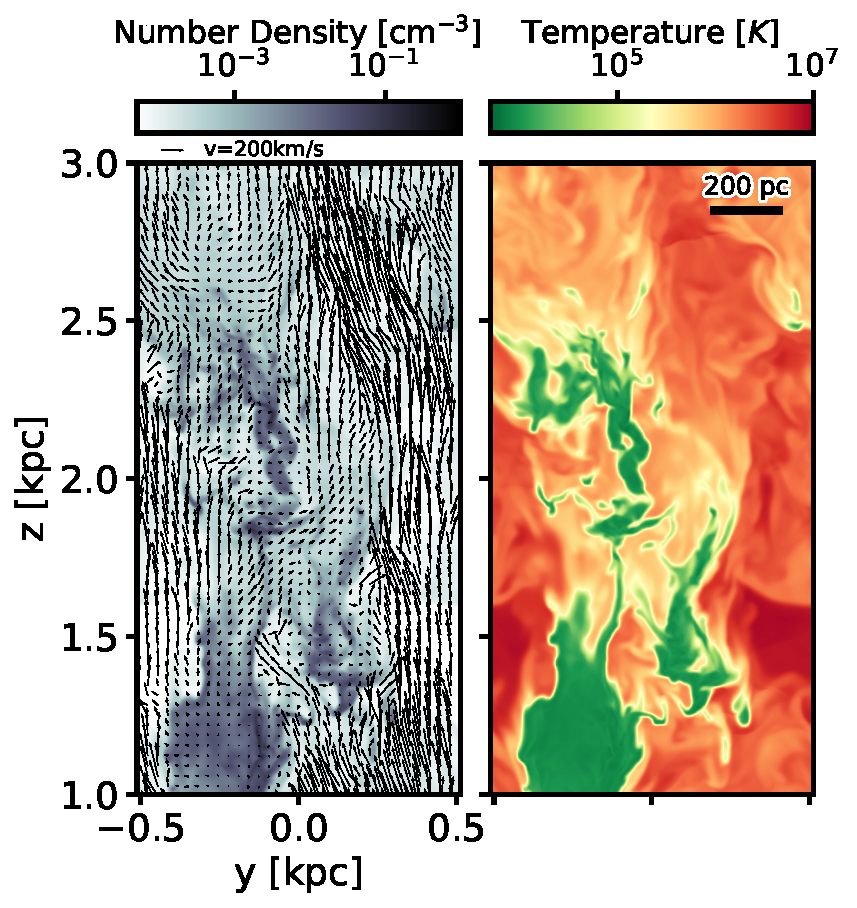
\includegraphics[width=\columnwidth]{slices_nH_T.pdf}
	\caption{Sample slices at $t=440\Myr$ through $x=140\pc$ showing number density (left panel) and  temperature (right panel) distribution for $z>1\kpc$. The arrows overlapping the density distribution represent the gas velocity field. Arrow lengths indicate velocity magnitudes. The multiphase nature of the outflowing gas is clearly visible in this figure. Slow-moving warm and dense clouds are surrounded by fast-moving hot and rarefied gas, with intermediate temperature gas at interfaces and wakes.} 
	\label{fig:slicenT}
\end{figure}

\begin{figure} 
	\centering
	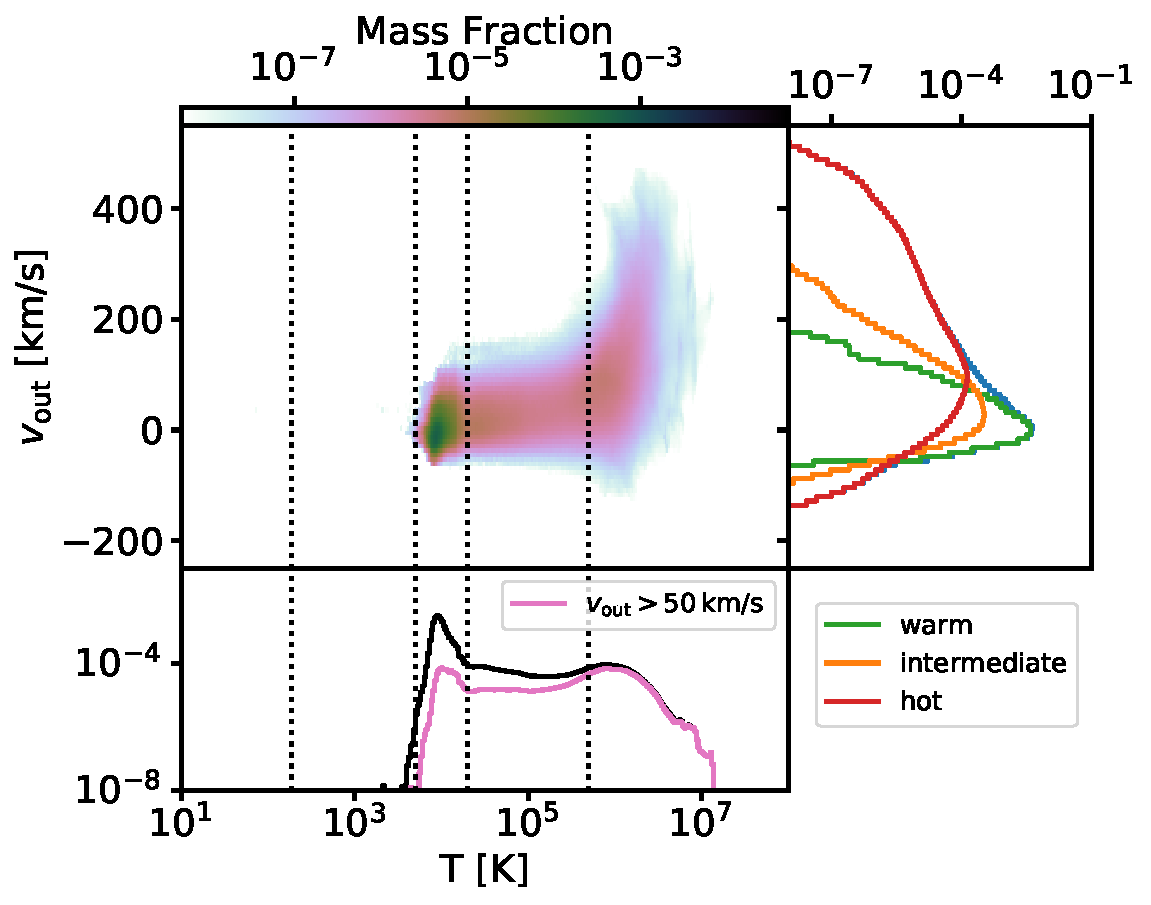
\includegraphics[width=\columnwidth]{pdfs.pdf}
	\caption{Mass-weighted PDF of the high-altitude gas ($z>1\kpc$) from the snapshot at $t=440\Myr$ in the temperature and outflow velocity ($v_{\rm out} \equiv v_z{\rm sign}(z)$) plane. The vertical dotted lines show the demarcation of the thermal phases. In the right panel, we present the temperature-integrated PDF (outflow velocity PDF). In the bottom panel, we present the velocity-integrated PDF (temperature PDF). For references, we also show the phase-separated velocity PDFs in the right panel and velocity-selected ($v_{\rm out}>50\kms$) temperature PDF in the bottom panel.}
	\label{fig:pdfs}
\end{figure}

\subsection{Time Evolution}\label{subsec:tigress_time_evol}

\begin{figure*}
    \centering
    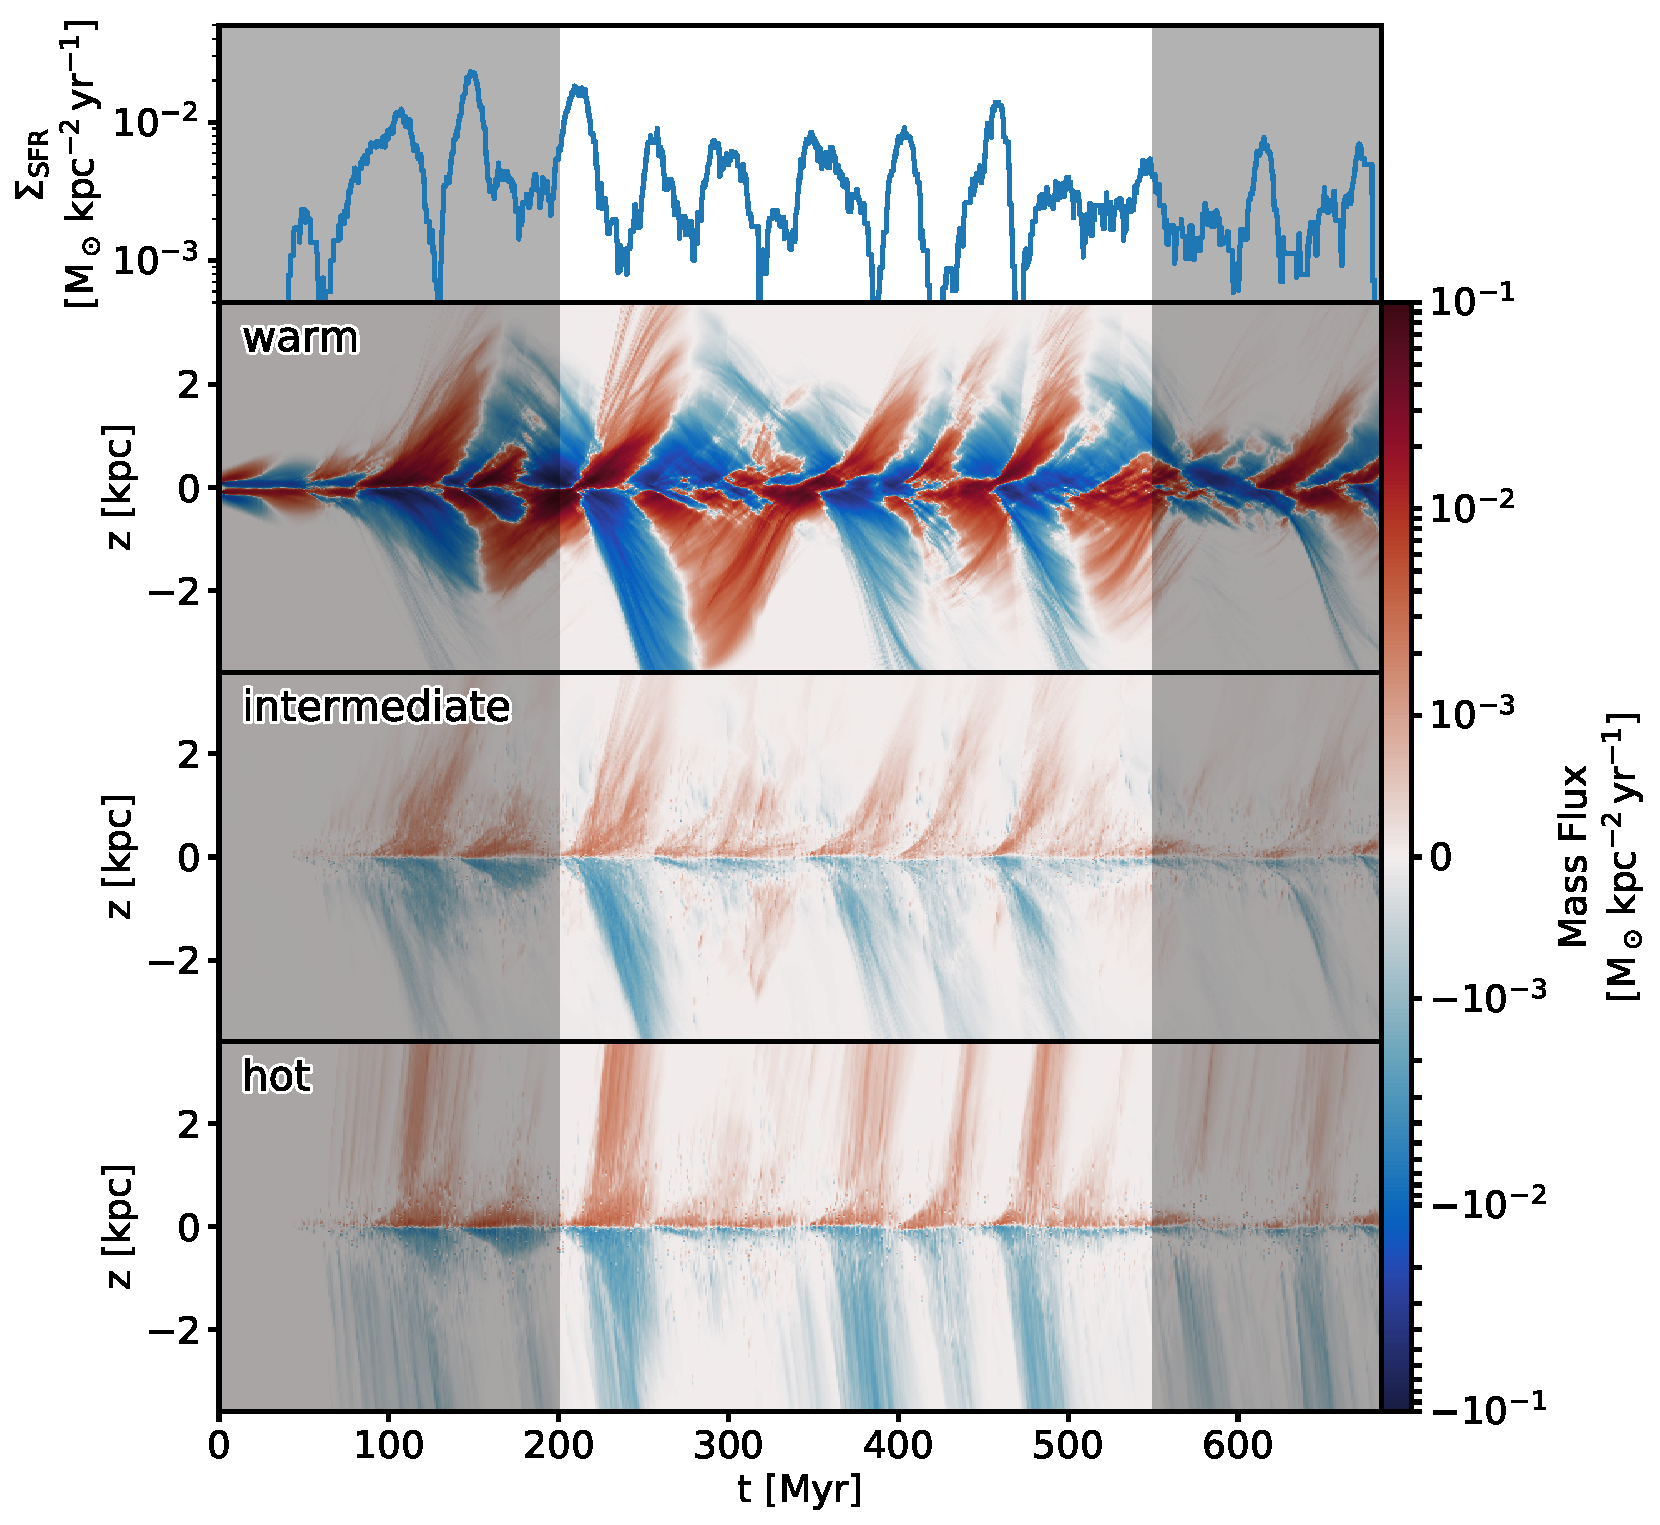
\includegraphics[width=\textwidth]{Mflux_tz.pdf}
    \caption{Space-time diagram of mass fluxes for warm, intermediate, and hot phases (bottom three panels) along with the SFR surface density (top panel). We analyze the simulation in $t=200-550\Myr$ (gray shaded regions are not included in the analysis). Star formation is bursty, with a period of $40-50\Myr$ corresponding to the vertical oscillation time scales of the diffuse warm/cold medium. The mean value of star formation rate surface density is well defined within the analyzed time range (secular variation is about 20\% of the mean); the 16th, 50th, and 84th percentiles of the SFR surface density are $\Sigma_{\rm SFR} = 2.8^{+4.2}_{-1.5}\times10^{-3}\sfrunit$.}
    \label{fig:mflux}
\end{figure*}

Now we build horizontally-averaged profiles to understand the overall time evolution of gas flows. For each thermal phase, the horizontal average of a quantity $q$ is defined by
\begin{equation}\label{eqn:havg}
\overline{q}_{\rm ph}(z;t) = \frac{\sum_{x,y} q(x,y,z;t)\Theta_{\rm ph}(T(x,y,z;t)) \Delta x \Delta y}{L_x L_y},
\end{equation}
where $\Theta_{\rm ph}(T)$ is the Heaviside step function that returns 1 for the gas temperature within the corresponding temperature range of the phase (ph = warm, intermediate, or hot) or 0 otherwise, $\Delta x = \Delta y =4\pc$ is the cell size, and $L_x=L_y=1024\pc$ is the horizontal domain size.

Figure~\ref{fig:mflux} shows time evolution of horizontally-averaged mass fluxes $\overline{\rho v_z}$ for the warm, intermediate, and hot phases. The red/blue color denote positive/negative mass flux and outflow/inflow for the gas  above the midplane $z>0$ (the opposite is true for the lower half of the disk, $z<0$). The time evolution of the warm mass at a given height is always alternating color, evidencing that the majority of the warm outflow falls back eventually (fountains) since it has launched with velocity that is insufficient to escape. By contrast, the hot gas has launched with high velocity and escapes the simulation domain (winds), keeping the mass flux nearly constant. The intermediate gas do not show clear evidence of subsequent inflows after outflows, but the mass flux is decreasing (color dilutes), implying the phase transition to the warm medium due to short cooling time of the intermediate temperature gas.

We also present time evolution of the SFR surface density measured from the mass of star clusters younger than 10~Myr on top of the space-time diagrams in Figure~\ref{fig:mflux}. Star formation is bursty, involving an order of magnitude level fluctuations. However, the system approaches a quasi-equilibrium, self-regulated state, meaning that the mean properties do not show a strong secular evolution. We select time range of $t=200-550\Myr$ for analysis, covering many feedback cycles and outflow events to investigate the outflow properties in the statistical steady state. The mean SFR surface density is decreased by 20\% within this time range as the system continuously lost the gas mass.

Within the time range of interests ($t=200-550\Myr$), we can identify 7-8 star formation peaks. However, from the mass flux evolution, there are only four clear breakouts (strong mass outflows in all phases). Two star burst events near $t\sim300\Myr$ do not result in strong outflows. We can see some hints of outflows for these events, but they fail to break out as the overall gas scale height has increased due to the earlier, stronger event at $t\sim 200\Myr$. The significant amount of material lifted upward is falling back during subsequent, relatively weak star formation events at $t\sim 250$ and $300\Myr$ and preventing breakouts from those events. This trend is generally true that outflows driven by the current star formation have to fight with inflows induced by the previous star formation. Succession of breakout is a very complicated consequence of spatial and temporal correlations of SNe themselves and with the gas.

\subsection{Time Averaged Properties}\label{subsec:tigress_tavg}
Despite of large temporal fluctuations, overall evolution reaches a quasi-steady state and we can investigate the time-averaged quantities to understand mean behavior. We use simulation outputs between 200 and 550 Myr to construct time averaged profiles as
\begin{equation}\label{eqn:tavg}
\abrackets{q}_{\rm ph}(z) = \frac{\sum_{t} \overline{q}_{\rm ph}(z;t)\Delta t}{t_{\rm bin}},
\end{equation}
where $t_{\rm bin} = 350\Myr$ and $\Delta t = 1\Myr$ is the time interval of the output dump.

To understand kinematics and dynamics of outflowing gas, it is crucial to understand the contribution of the each component in the momentum equation.\footnote{Note that, for simplicity, we dropped the Coriolis force and tidal potential terms arising from the galactic differential rotation included in the simulation. \citet{Kim&Ostriker18} presents full equations, analyzes each term, and concludes that these have negligible impacts on the outflows we are analyzing in this paper. Note also that on the RHS of the equation (14) in \citet{Kim&Ostriker18}, $\Phi_{\rm tot}\divergence{\rho\vel}$ is missed.} By taking horizontal and temporal averages, we obtain the steady-state vertical momentum equation as
\begin{equation}\label{eqn:mom}
\begin{split}
 \deriv{}{z}\sum_{\rm ph} \abrackets{P_{\rm turb,z} + P_{\rm th} + \Pi_{\rm mag,z}}_{\rm ph} = \\
-\sum_{\rm ph} \abrackets{\rho\rbrackets{\deriv{\Phi_{\rm ext}}{z} +\deriv{\Phi_{\rm sg}}{z}}}_{\rm ph},   
\end{split}
\end{equation}
where the three terms on the left hand side are
turbulent, thermal, and magnetic components of the pressure gradient force, respectively, and the two terms on the right hand side are external and self gravity, respectively. $\Phi_{\rm ext}$ is the gravitational potential due to old stellar disk and dark matter halo as prescribed in Equation (\ref{eqn:pot}), and $\Phi_{\rm sg}$ is the gravitational potential of gas itself (including negligible young star clusters) obtained by solving the Poisson's equation.  The thermal and turbulent ``support'' equals to thermal pressure ($P_{\rm th }$) and vertical turbulent pressure\footnote{The term ``turbulent'' may be confusing since at high altitudes the gas motion is more or less ordered, dominated by either outflow or inflow at a given time. However, the inflow and outflow coexist and alternate with time. Therefore, the horizontally and temporally averaged pressure we consider arises from a variance of vertical velocity, although there is a significant contribution from the ram pressure. For simplicity, we rather not to separate them and use the term ``turbulent pressure'', which is still a fair nomenclature.} ($P_{\rm turb,z}=\rho v_z^2$), respectively, but the magnetic ``support'' ($\Pi_{\rm mag}$) is smaller than the magnetic pressure ($P_{\rm mag} = (B_x^2+B_y^2+B_z^2)/(8\pi)$) due to the magnetic tension term ($-B_z^2/(4\pi)$), resulting in $\Pi_{\rm mag}= (B_x^2+B_y^2-B_z^2)/(8\pi)$.

By integrating Equation (\ref{eqn:mom}) from the top/bottom of the simulation domain to the height $z$, we can rewrite the equation in terms of the momentum flux difference (or vertical support) and the weight of gas
\begin{equation}\label{eqn:mom2}
\sum_{\rm ph} \sbrackets{ \mathcal{F}_{\rm p, ph} (z)- \mathcal{F}_{\rm p, ph} (\pm L_z/2)}
= \sum_{\rm ph} \mathcal{W}_{\rm ph}(z),
\end{equation}
where the total momentum flux at $z$ is defined by
\begin{equation}\label{eqn:Fp}
\mathcal{F}_{\rm p, ph}(z) \equiv \abrackets{P_{\rm turb,z} + P_{\rm th} + \Pi_{\rm mag,z}}_{\rm ph}(z),
\end{equation}
and the total weight of gas is defined by
\begin{equation}\label{eqn:weight}
\mathcal{W}_{\rm ph}(z) \equiv \int_{\pm L_z/2}^z \abrackets{\rho\rbrackets{\deriv{\Phi_{\rm ext}}{z} +\deriv{\Phi_{\rm sg}}{z}}}_{\rm ph} dz \,.
\end{equation}


Figure~\ref{fig:vertical_equilibrium}(a) compares the momentum flux difference (the LHS of Equation~(\ref{eqn:mom2})) and the weight of gas (the RHS of Equation~(\ref{eqn:mom2})). For the gas as a whole, on average, the vertical dynamical equilibrium holds (the vertical support equals the weight of gas) very well as shown in previous work \citep[e.g.,][]{KOK13,KO15b}. This again justifies the quasi-steady state assumption. We also show that the weight of gas is mostly due to the external gravity, especially above the gas scale height. In the panels (b) and (c), we decompose the momentum flux difference and weight into different thermal phases. Since the warm gas dominates mass fraction in the simulation, the weight is dominated by the warm medium everywhere, while the vertical support comes from both warm and hot phases comparably, especially at high-$|z|$. By comparing the vertical support and weight individually, the warm gas is lacking in the support, while the hot gas shows large excess in the support. The support and weight of the intermediate phase are roughly balanced within the phase without significant excess or deficit.

In order to anatomy the vertical support further, we construct averaged profiles of individual pressure/support components and phases. Figure~\ref{fig:mean_profiles} shows the horizontally and temporally averaged profiles of the vertical (a) thermal, (b) turbulent, and (c) magnetic support for different thermal phases. Near the midplane $|z|<H$, the majority of support arises from the warm phase, and all thermal, turbulent, and magnetic components of the warm phase are comparable with each other. The hot component also contributes significant thermal pressure in this region. At the high-altitude $|z|>(1-2)H$, the hot gas dominates both thermal and turbulent pressures. The turbulent pressure of the warm phase is also substantial, but drops rapidly as the warm outflow falls back at $z\sim1-2\kpc$ (see Figure~\ref{fig:mflux}). However, as shown in Figure~\ref{fig:vertical_equilibrium}(b), the ``support'' from hot and warm phases are similar in this region, since the support arises from the momentum flux ``difference''. Because of this, although the intermediate phase pressures are always negligible in terms of the absolute values, the vertical support is not negligible (but the support of the intermediate phase is mostly compensated by its own weight; see Figure~\ref{fig:vertical_equilibrium}(b) and (c)). The mangetic component is negligible in the high-$|z|$ region so that we  safely ignore the magnetic field contribution in the following analysis.

\begin{figure*}
	\centering
 	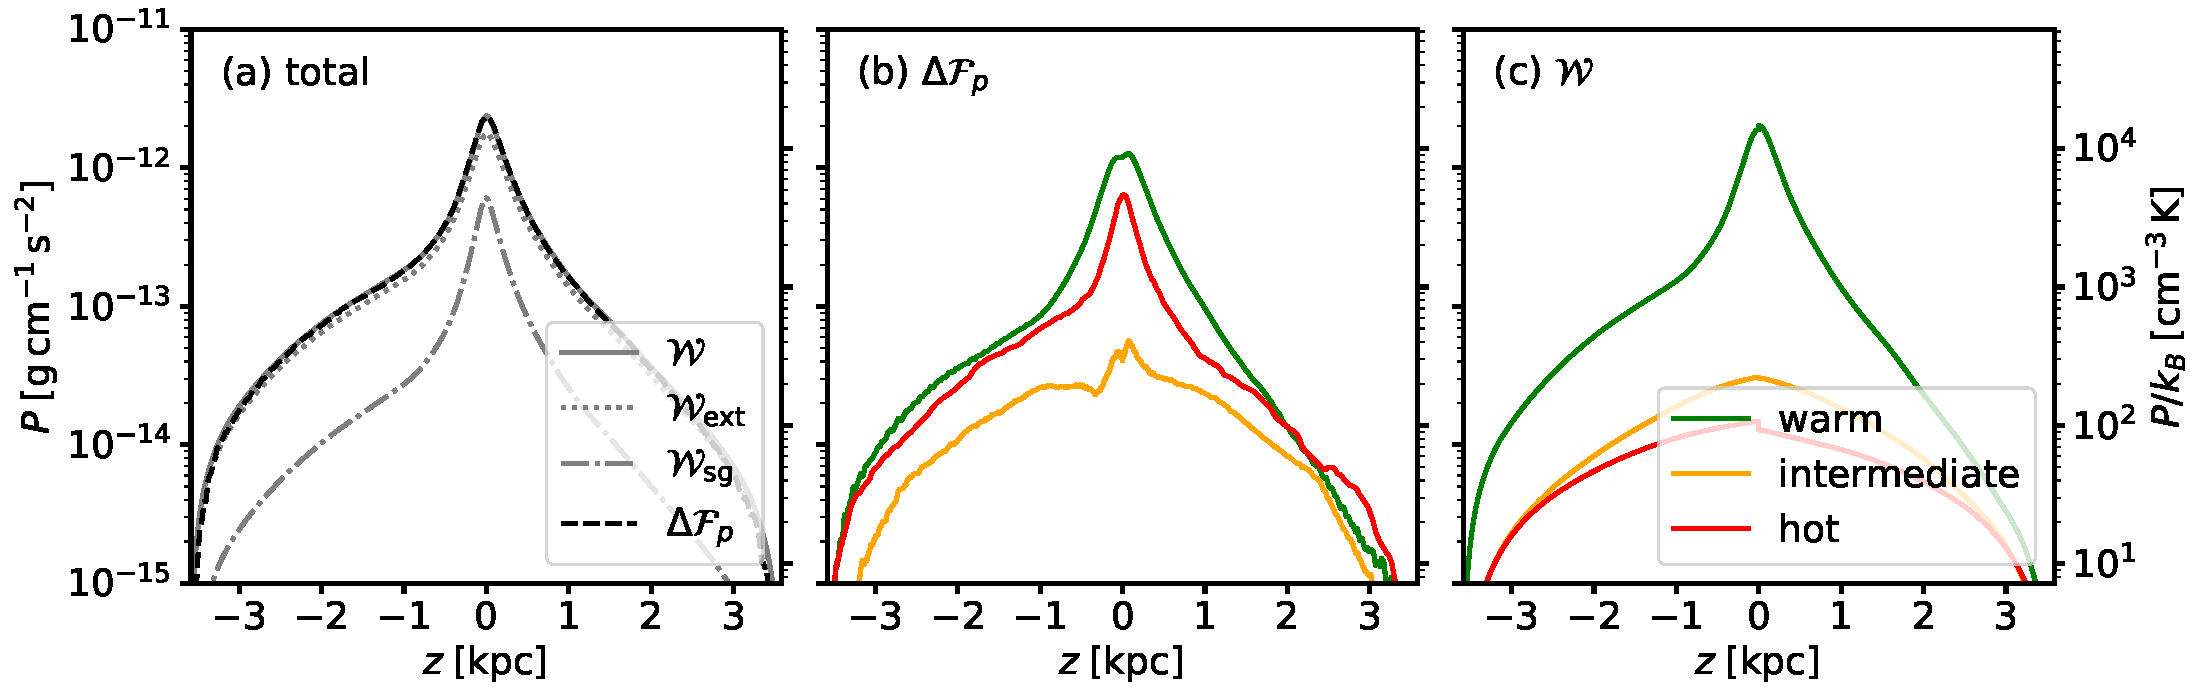
\includegraphics[width=\textwidth]{vertical_equilibrium.pdf}
	\caption{{\bf (a)} The total momentum flux difference (or vertical support; the LHS of Equation (\ref{eqn:mom2})) and the weight of gas (the RHS of Equation (\ref{eqn:mom2})) as a function of $z$. The almost perfect agreement between two curves demonstrate the validity of the vertical dynamical equilibrium. The weight is further decomposed into the contribution from external (dotted) and self (dot-dashed) gravity terms, showing the dominance of the external gravity term. We also show the phase-separated {\bf (b)} the momentum flux differences and {\bf (c)} the weight.}
	\label{fig:vertical_equilibrium}
\end{figure*}

\begin{figure*}
	\centering
    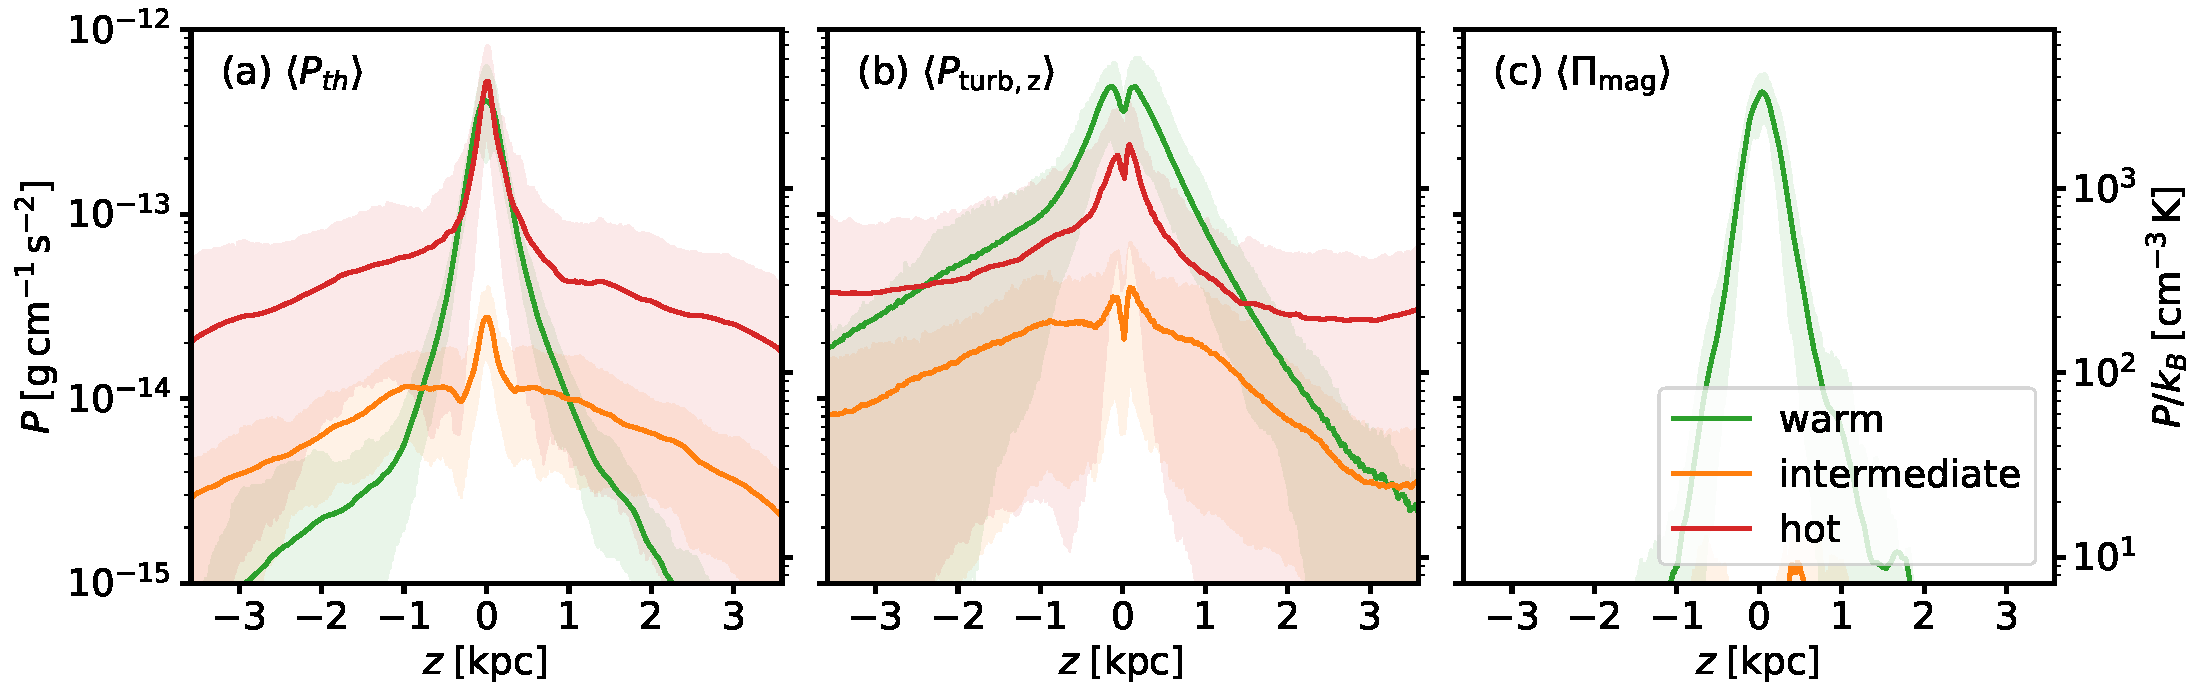
\includegraphics[width=\textwidth]{mean_profiles.pdf}
	\caption{Horizontally and temporally averaged vertical profiles of {\bf (a)} thermal pressure $\abrackets{P_{\rm th}}$, {\bf (b)} turbulent pressure $\abrackets{P_{\rm turb,z}}$, and {\bf (c)} magnetic support $\abrackets{\Pi_{\rm mag}}$.  The warm, intermediate, and hot phases are color coded by green, yellow, and red, respectively. The shaded area covers the 16th and 84th percentiles of temporal fluctuations. } 
	\label{fig:mean_profiles}
\end{figure*}

%%CGK: Now I'm not sure we definitely need this since it does not add significant information.

Figure~\ref{fig:typical_profiles} shows ``typical vertical support'' of each component and each phase, dividing the mean support by the area fraction $f_{\rm A,ph}\equiv\abrackets{1}_{\rm ph}$. For example, $\tilde{P}_{\rm th}\equiv\abrackets{P_{\rm th}}/f_{\rm A,ph}$. In contrast to Figure~\ref{fig:mean_profiles}, these profiles show the relative importance of each of the three components in the vertical support for a particular phase. Interestingly, the typical turbulent pressure of the warm medium is the largest and nearly constant with respect to the height. Combining with the observation of Figure~\ref{fig:mean_profiles}, the contribution of the warm to the total support drops rapidly since the area fraction drops as more and more warm medium falls back. This figure reinforces the conclusions from Figure~\ref{fig:mean_profiles}: (1) for the warm phase, all thermal, turbulent, and magnetic components are comparable near the midplane, but turbulent pressure dominates at high-altitude, (2) the hot gas has comparable thermal and turbulent pressures at all heights, and (3) magnetic support is negligible at high altitude.

\begin{figure*}
	\centering
    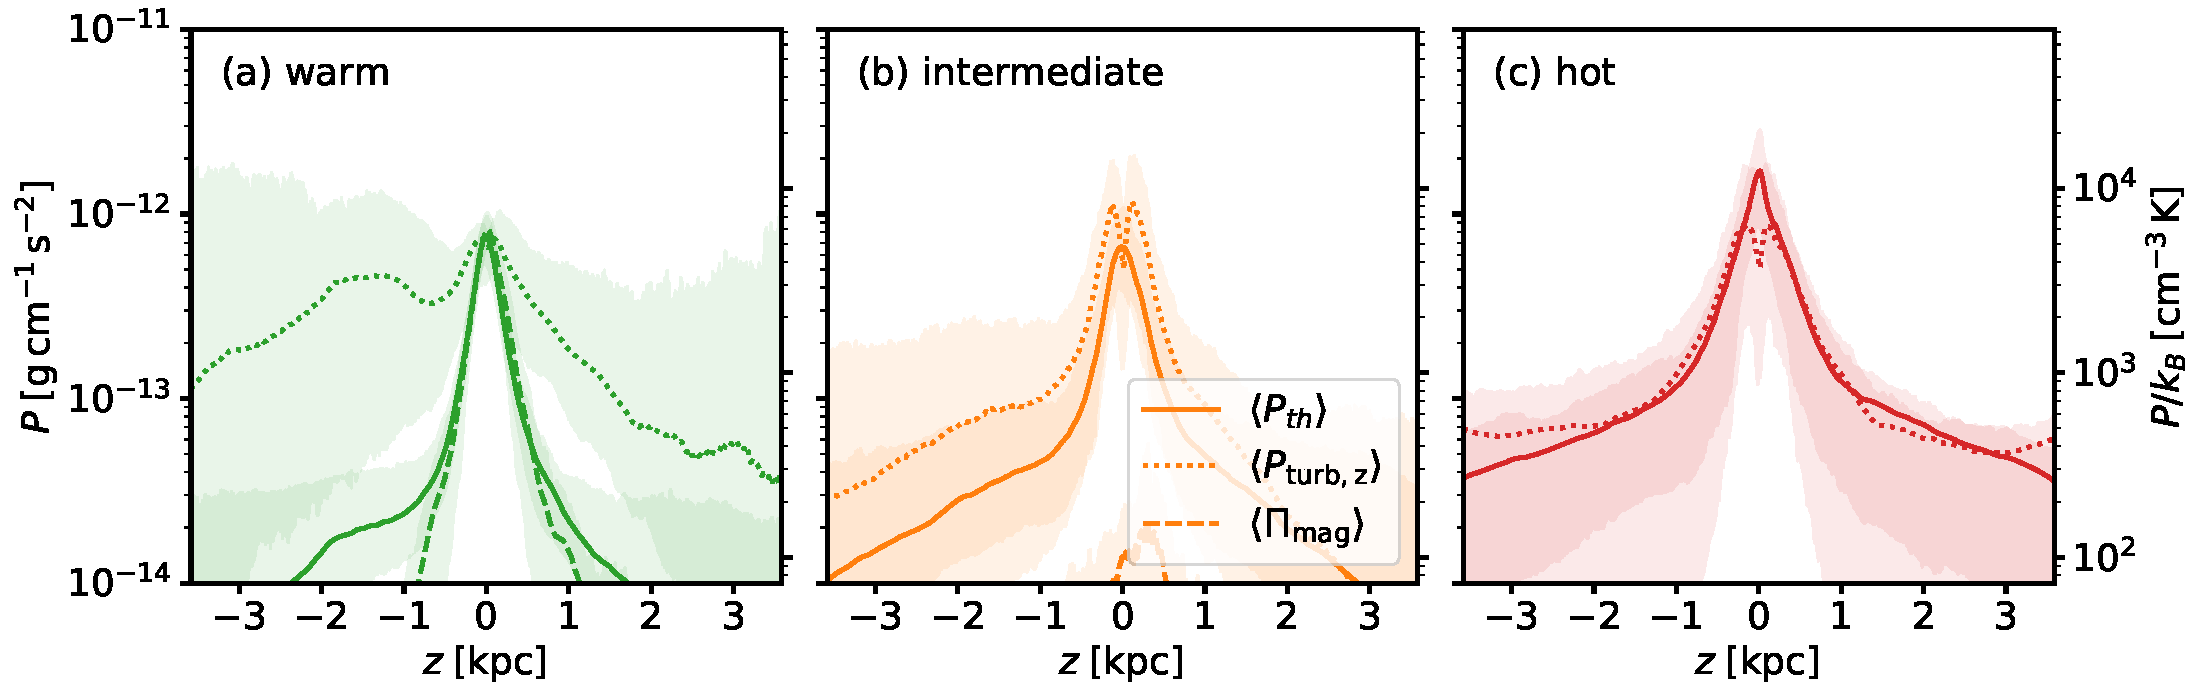
\includegraphics[width=\textwidth]{typical_profiles.pdf}
	\caption{Vertical profiles of typical thermal pressure ($\tilde{P}_{\rm th}$; solid), turbulent pressure ($\tilde{P}_{\rm turb,z}$; dotted) and magnetic support ($\tilde{\Pi}_{\rm mag}$; dot-dashed) for the {\bf (a)} warm, {\bf (b)} intermediate, and {\bf (c)} hot  phases. The shaded area covers the 16th and 84th percentiles of temporal fluctuations. Note that the averaged profiles shown in Figure~\ref{fig:mean_profiles} can be obtained by multiplying the area fraction of each phase $f_{\rm A,ph}=\abrackets{1}_{\rm ph}$, e.g., $\abrackets{P}_{\rm th} = f_{\rm A,ph}\tilde{P}_{\rm th}$.} 
	\label{fig:typical_profiles}
\end{figure*}

\section{Ballistic Model of the Warm Outflow}\label{sec:ballistic}

\subsection{Ballistic Model}\label{subsec:bal_model}
To describe the evolution of the warm outflow shown in Figure~\ref{fig:slicenT}, we first consider the simplest model, namely a ballistic model given by the conservation of the mechanical energy; $v_z^2/2 + \Phi = \textrm{constant}$. The ballistic model assumes that each warm gas entity evolves independently and the change of its velocity is solely due to the gravity (no hydrodynamic interactions). Note that the external gravity dominates at the high-altitudes so that $\Phi\approx\Phi_{\rm ext}$ is a good assumption. Since $\Phi_{\rm ext}$ is known and fixed in time (see Equation (\ref{eqn:pot})), we can easily calculate the vertical velocity of the warm outflow at arbitrary height $z$ from the conditions at launching ($z=z_i$) as
\begin{equation}\label{eqn:bal_vf}
v_z (z) = \pm \sqrt{v_i^2 -2\rbrackets{\Phi (z) - \Phi (z_i)}}\,
\end{equation}
where $v_i = v_z(z_i)$ is the vertical velocity at launching. 

Since the outflowing gas in the simulation is not launched with a single velocity, it is more informative to consider a velocity probability distribution function (v-PDF). In order to predict the mass-weighted v-PDF, $dM/dv$, at a height $z$, we consider the conservation of the mass flux for each velocity element. The mass of gas in a range of a velocity range between $v_0$ and $v_0+\delta v_0$ is given by
\begin{eqnarray}
\delta M(v_0) = \deriv{M}{v}\Big|_{v_0}  \delta v_0,
\end{eqnarray}
while the total mass flux $\rho v$ can be written as
$\delta M(v_0)v_0/(A\delta z)$
where $A\delta z$ is a volume of a thin slab that the gas passes through. Assuming the mass flux conservation of the velocity element as it travels from $z_i$ to $z_f$, the change of velocity from $v_i$ to $v_f=v_z(z_f)$ yields
\begin{eqnarray}\label{eqn:Mv}
\deriv{M}{v}\Big|_{v_f} v_f \delta v_f = \deriv{M}{v}\Big|_{v_i} v_i\delta v_i\,.
\end{eqnarray}
From Equation (\ref{eqn:bal_vf}), we have $v_f \delta v_f = v_i\delta v_i$, and Equation~\ref{eqn:Mv} simply becomes
\begin{eqnarray}\label{eqn:vpdf}
\deriv{M}{v}\Big|_{v_f} = \deriv{M}{v}\Big|_{v_i}\,.
\end{eqnarray}
Therefore, under the assumption of the mass flux conservation for each velocity element, the velocity distribution at $z_{f}$ can be obtained by shifting the initial velocity distribution at $z_{i}$ according to the ballistic equation (Equation (\ref{eqn:bal_vf})).


\subsection{Comparison Between Simulation and Model}\label{subsec:bal_comparison}
\begin{figure*}
	\centering
	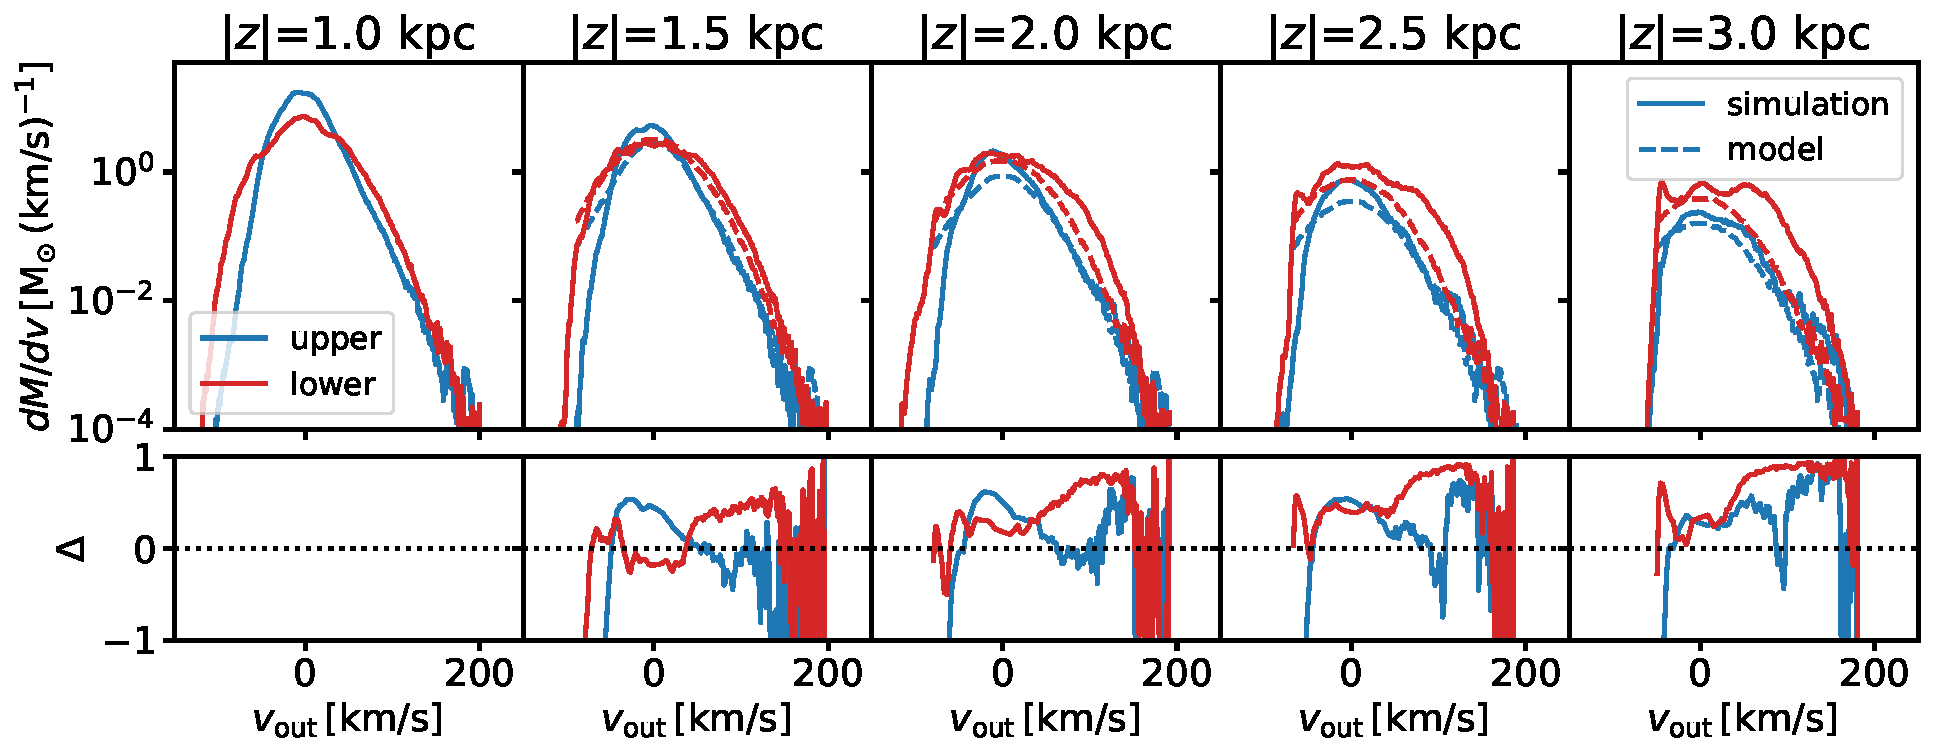
\includegraphics[width=\textwidth]{ballistic_warm.pdf}
	\caption{The mass-weighted velocity PDFs for the warm phase along with the fractional difference between the simulation data and the ballistic model, $\Delta=$ (Simulation - Model)/Simulation in the bottom. From left to right, we show the v-PDFs from the simulation data at $|z|=1$, 1.5, 2, 2.5, and 3~kpc as solid lines for the upper (blue) and lower (orange) disks. Note that the vertical velocity is multiplied by the sign of $z$ to convert it to the outflow velocity. For $|z|>1$, we plot the ballistic model prediction (see Section~\ref{subsec:bal_model}) as the dashed line adopting the v-PDF at $|z|=1\kpc$ as an initial condition.
 } 
	\label{fig:ballistic_warm}
\end{figure*}

\begin{figure*}
	\centering
	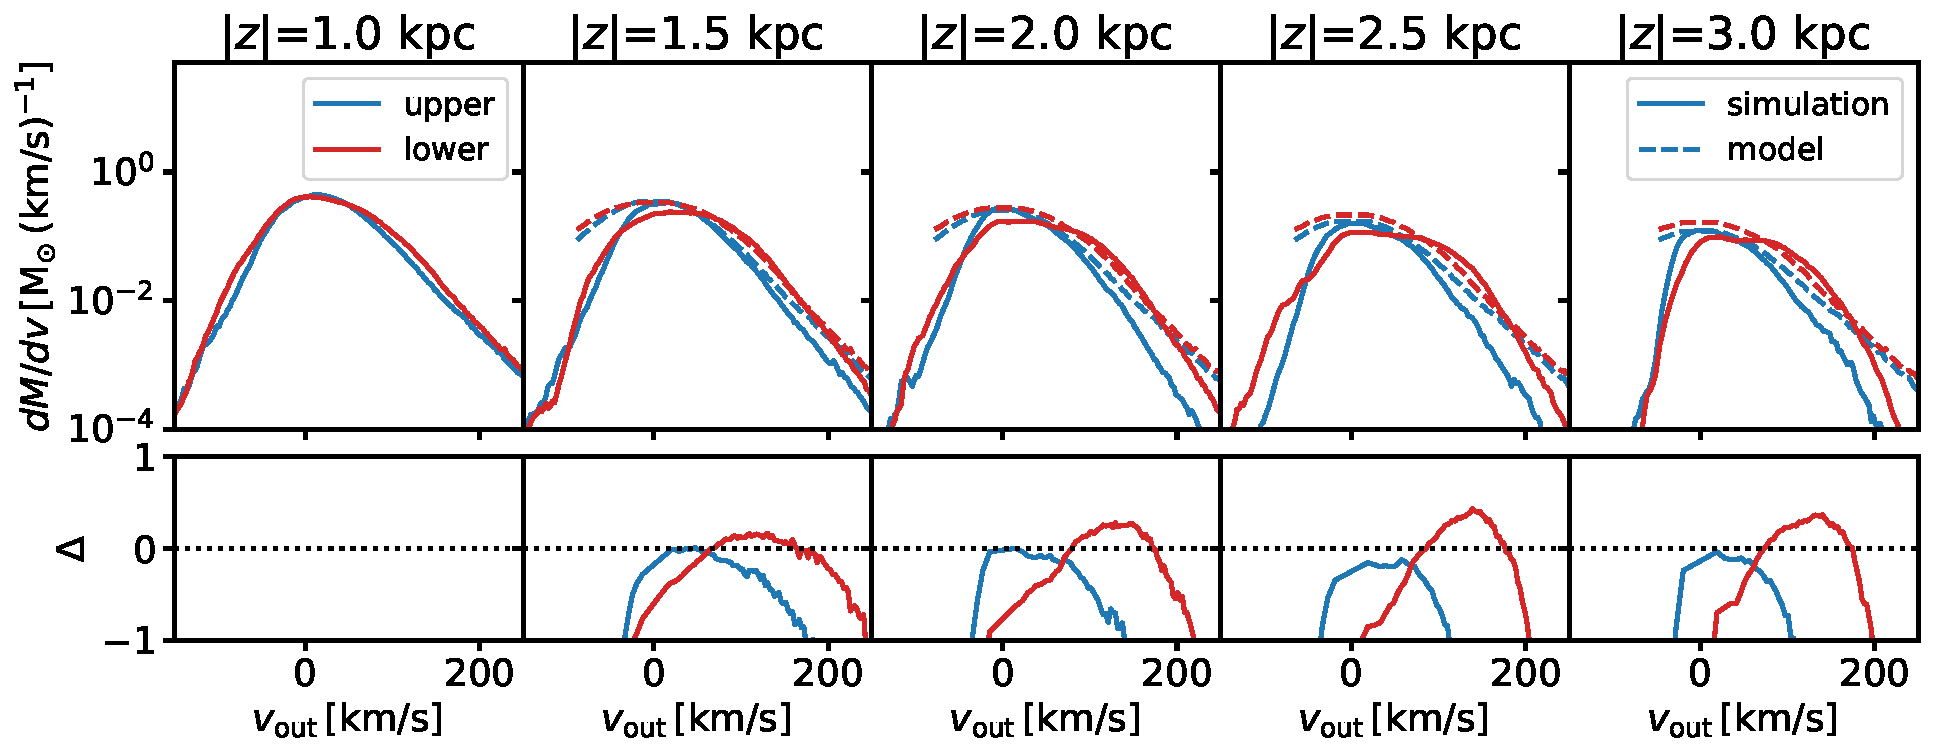
\includegraphics[width=\textwidth]{ballistic_int.pdf}
	\caption{Same as Figure~\ref{fig:ballistic_warm}, but for the intermediate phase.} 
	\label{fig:ballistic_int}
\end{figure*}

\begin{figure*}
	\centering
	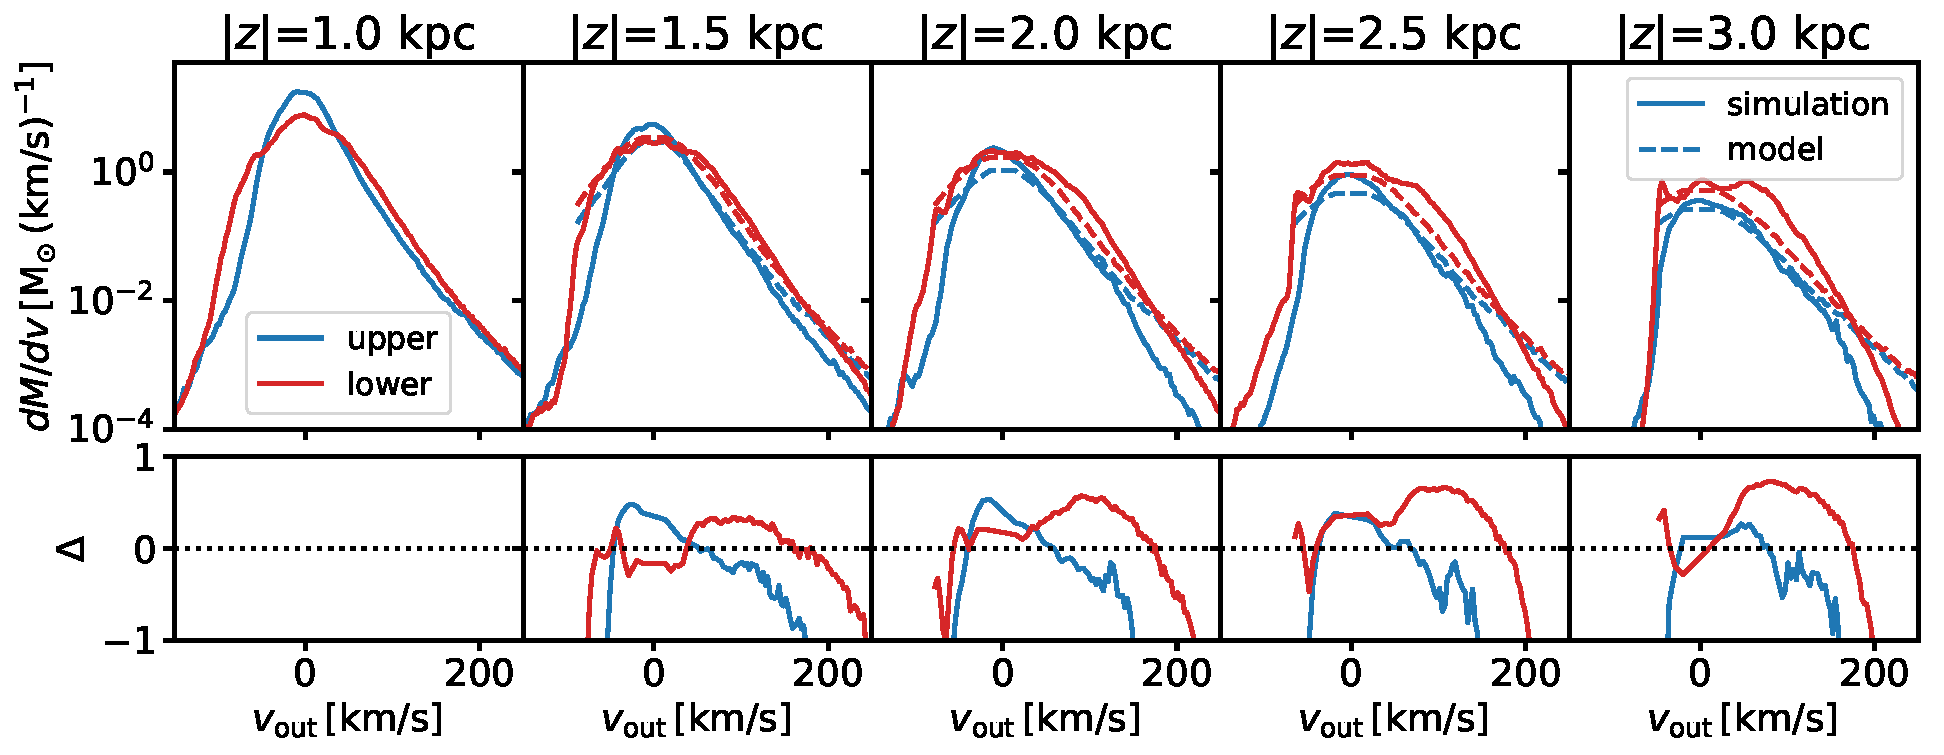
\includegraphics[width=\textwidth]{ballistic_warm_int.pdf}
	\caption{Same as Figure~\ref{fig:ballistic_warm}, but for the sum of the warm and intermediate phases.} 
	\label{fig:ballistic_warm_int}
\end{figure*}

Since the typical turbulent pressure of the warm phase is the largest among all the momentum flux terms and phases (see Figure~\ref{fig:typical_profiles}), the warm outflow would indeed evolve more or less ballistically without altering its trajectory by other phases. Therefore, the warm phase is the most suitable component to be compared with the ballistic model.

We compare the mass-weighted v-PDFs of the warm phase as a function of height obtained from the simulation with those predicted by the ballistic model (Section~\ref{subsec:bal_model}). For simulation snapshots, we first calculate the mass-weighted v-PDF at each height $z$ and take time averages. For the ballistic model, we use the v-PDF at $|z_i|=1\kpc$ from the simulation as an initial (launching) condition and calculate the predicted v-PDF using at heights $|z_f|=1.5$, 2, 2.5, and 3$\kpc$ based on Equations (\ref{eqn:bal_vf}) and (\ref{eqn:vpdf}). Note that we treat the upper ($z>0$) and lower ($z<0$) sides of the simulation domain independently. Assuming steady injection of the outflowing gas through the $z=z_i$ plane, both outflowing and inflowing components of the v-PDF at different heights can be predicted (see $\pm$ signs in Equation (\ref{eqn:bal_vf})). Due to the limited vertical extent of the simulation, however, outflowing gas with sufficiently high speed is likely to exit the simulation box. Thus, for the fair comparison with the simulation, we set a cut-off velocity in the computation of the inflowing component; 
\begin{eqnarray}
|v_{\rm{cut}}| \equiv \sqrt{2\, \sbrackets{ \Phi(z_i) - \Phi(\pm L_z/2)}}=98\kms\,,
\end{eqnarray}
where $L_z$ is the vertical size of the simulation box.
 
Figure~\ref{fig:ballistic_warm} shows the comparison between simulation and model for the warm phase at heights above (blue) and below (red) the galactic plane, respectively.
The quantitative comparison between the simulation data (solid) and the ballistic predictions (dashed) is presented as the fractional difference in the respective bottom panels. The fractional difference is defined by 
\begin{equation}\label{eqn:delta}
\Delta\equiv \frac{dM/dv({\rm simulation}) - dM/dv({\rm model})}{dM/dv({\rm simulation})}.
\end{equation}
The positive or negative $\Delta$ means that the ballistic model under- or over-predicts the mass in a velocity bin, respectively.

Despite the highly simplistic assumptions applied here, the ballistic model generally recovers the v-PDF at different heights quite well. In order to construct the v-PDF from the ballistic model, we also neglect interaction between outflow and inflow within the phase, which certainly exists due to the bursty nature of the star formation and outflows (see Figure~\ref{fig:mflux}). Therefore, the overall agreement of the ballistic prediction to the simulation data gets worse as the distance between heights of launching and prediction gets larger and at higher outflow velocity bins. 

The ballistic model underestimates the mass of the warm phase at high velocity bins (positive $\Delta$ in Figure~\ref{fig:ballistic_warm}), without overestimation at low velocity bins (no significant negative $\Delta$ in Figure~\ref{fig:ballistic_warm}). This potentially means that the high velocity excess of the warm medium is not due to the acceleration of low velocity warm outflow itself but due to the addition of high velocity gas from the other phases. Regarding the short cooling time of the intermediate phase, it is natural to expect a phase transition from the intermediate phase to the warm phase. For the intermediate phase, the typical cooling time above $|z|>1\kpc$ is $t_{\rm cool}\equiv \abrackets{P_{\rm th}}/[(\gamma-1)\abrackets{\mathcal{L}}]\sim 1-100\Myr$, increasing from low-altitude to high-altitude. This is shorter than or comparable to the outflow crossing time for the simulation domain from $|z|=1\kpc$ to $|z|=L_z/2$, $t_{\rm cross}=(L_z/2 - 1\kpc)/v_{\rm out} = 12.5\Myr (v_{\rm out}/200\kms)^{-1}$.

To confirm this idea, we perform the same comparison for the intermediate phase in Figure~\ref{fig:ballistic_int}. 
Here, we do not anticipate the general validity of the ballistic model for the intermediate phase since the non-negligible cooling in the intermediate phase violates the necessary assumptions for the ballistic model (mass conservation). Note that, although the phase transition due to cooling of the intermediate phase also means the addition of the mass to the warm phase, the contribution from the intermediate phase is insignificant for the warm phase so that the ballistic assumption we made for the warm phase may still hold approximately. 

Bearing these caveats in mind, Figure~\ref{fig:ballistic_int} shows general deficits of the mass at high-velocity bins (negative $\Delta$), without significant excesses in any other velocity bins. The ``missing'' intermediate phase gas has to be added to the warm phase and can be responsible for the excess shown in Figure~\ref{fig:ballistic_warm}. Since the mass fraction at high-velocity bins is smaller, the excess would be more prominent at these bins.

If we simply assume that the gas at the intermediate temperature cools and turns into the warm phase, the phase transition just moves the mass at a given velocity bin from one phase to the other. As shown in Figure~\ref{fig:ballistic_warm_int}, when we consider both warm and intermediate phases together, the agreement gets only slightly better. Especially, the excess of the warm phase in the upper side of disk is well counterbalanced by the deficit of the intermediate phase. However, in the lower side of disk, the intermediate gas does not make the ballistic model better.

So far, we neglect any dynamical interaction between phases. But, the v-PDFs shown in Figures~\ref{fig:ballistic_warm}-\ref{fig:ballistic_warm_int}  possess a signature of phase interaction. The outflow is generally asymmetric (see Figure~\ref{fig:mflux}), and this is evident in Figure~\ref{fig:ballistic_warm}, where the v-PDFs of the warm phase at $|z|=1\kpc$ show significant difference. However, the intermediate phase shows very similar v-PDFs at $|z|=1\kpc$ for both sides. The asymmetry in the intermediate phase emerges as it moves outward and interacts with different warm phase outflows. In addition to the failure of the simple cooling idea, this clearly implies that the dynamical interaction between phases exists and affects the evolution of outflows noticeably. We quantify this effect in the next section.

%%%%%%%%%%%%%%%%%%%%%%%%%%%%%%%%%%%%%%%%%%%%%%%%%%%%%%%%%%%%%%%%%%%%%%%%%%%%%%%%%%%
\section{Mass, Momentum, and Energy Transfers Between Phases}\label{sec:flux_analysis}
\begin{figure*}
	\centering
	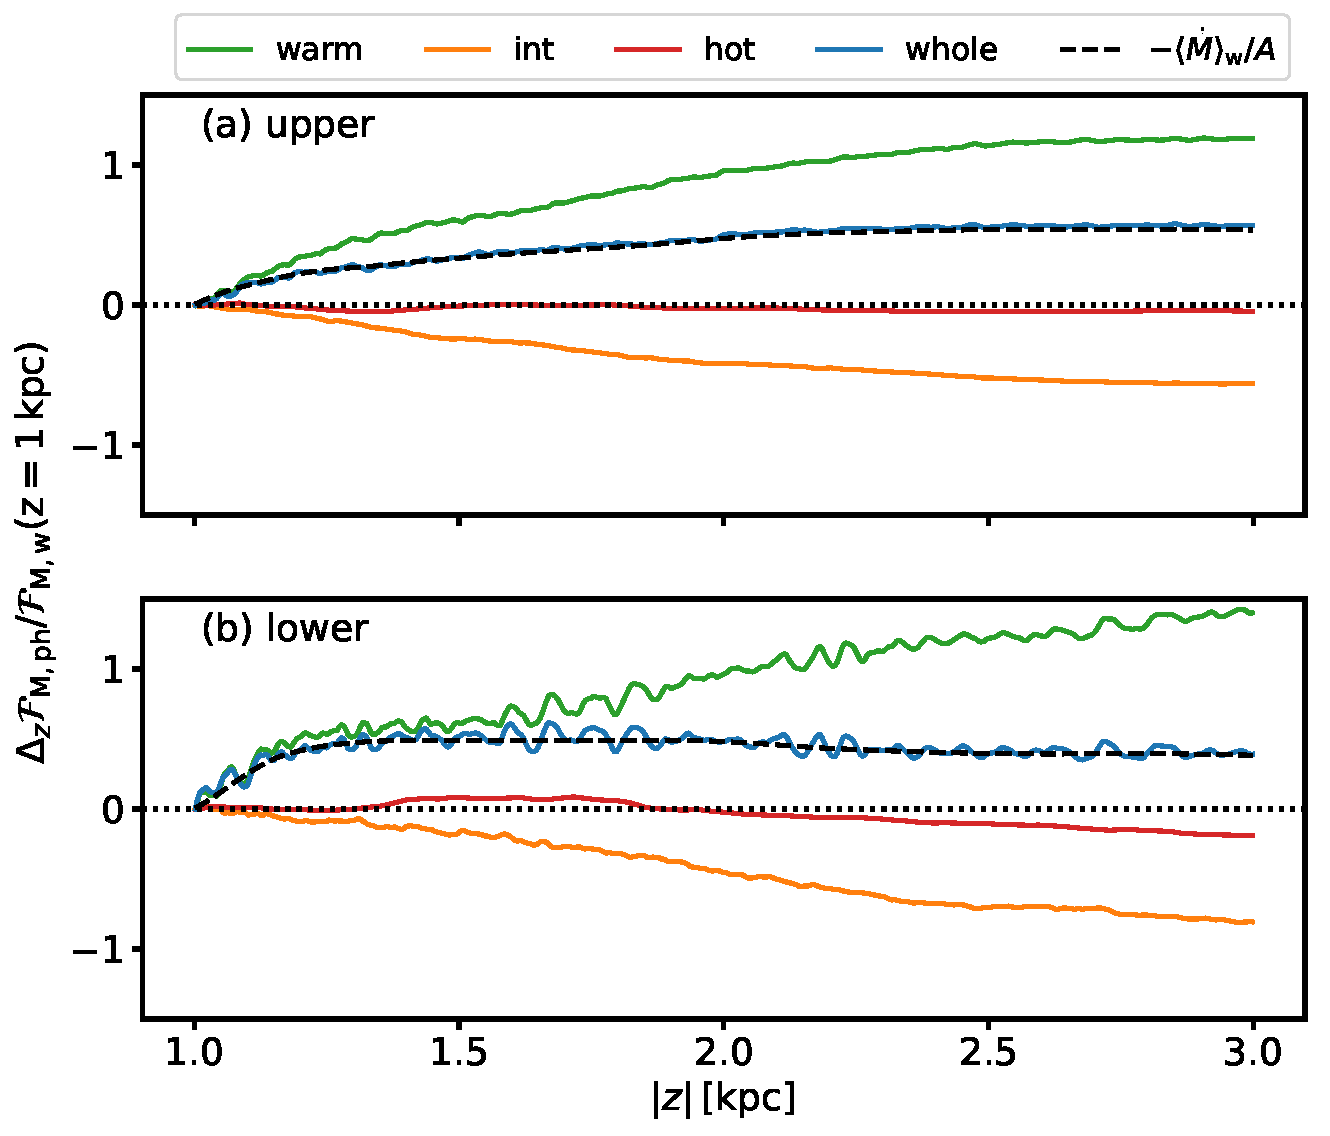
\includegraphics[width=0.9\textwidth]{mass_conservation.pdf}
	\caption{Mean mass flux differences of each thermal gas phase between the height of interest $z$ and launching $z_i=1\kpc$ from the {\bf (a)} upper and {\bf (b)} lower sides of the disk. The mass flux difference is normalized by the mass flux of the warm phase at $z=z_i$. The net mass change of the warm phase is shown as the black dashed line for a reference, which compensates the total flux difference.}
	\label{fig:mcons}
\end{figure*}
\begin{figure*}
	\centering
	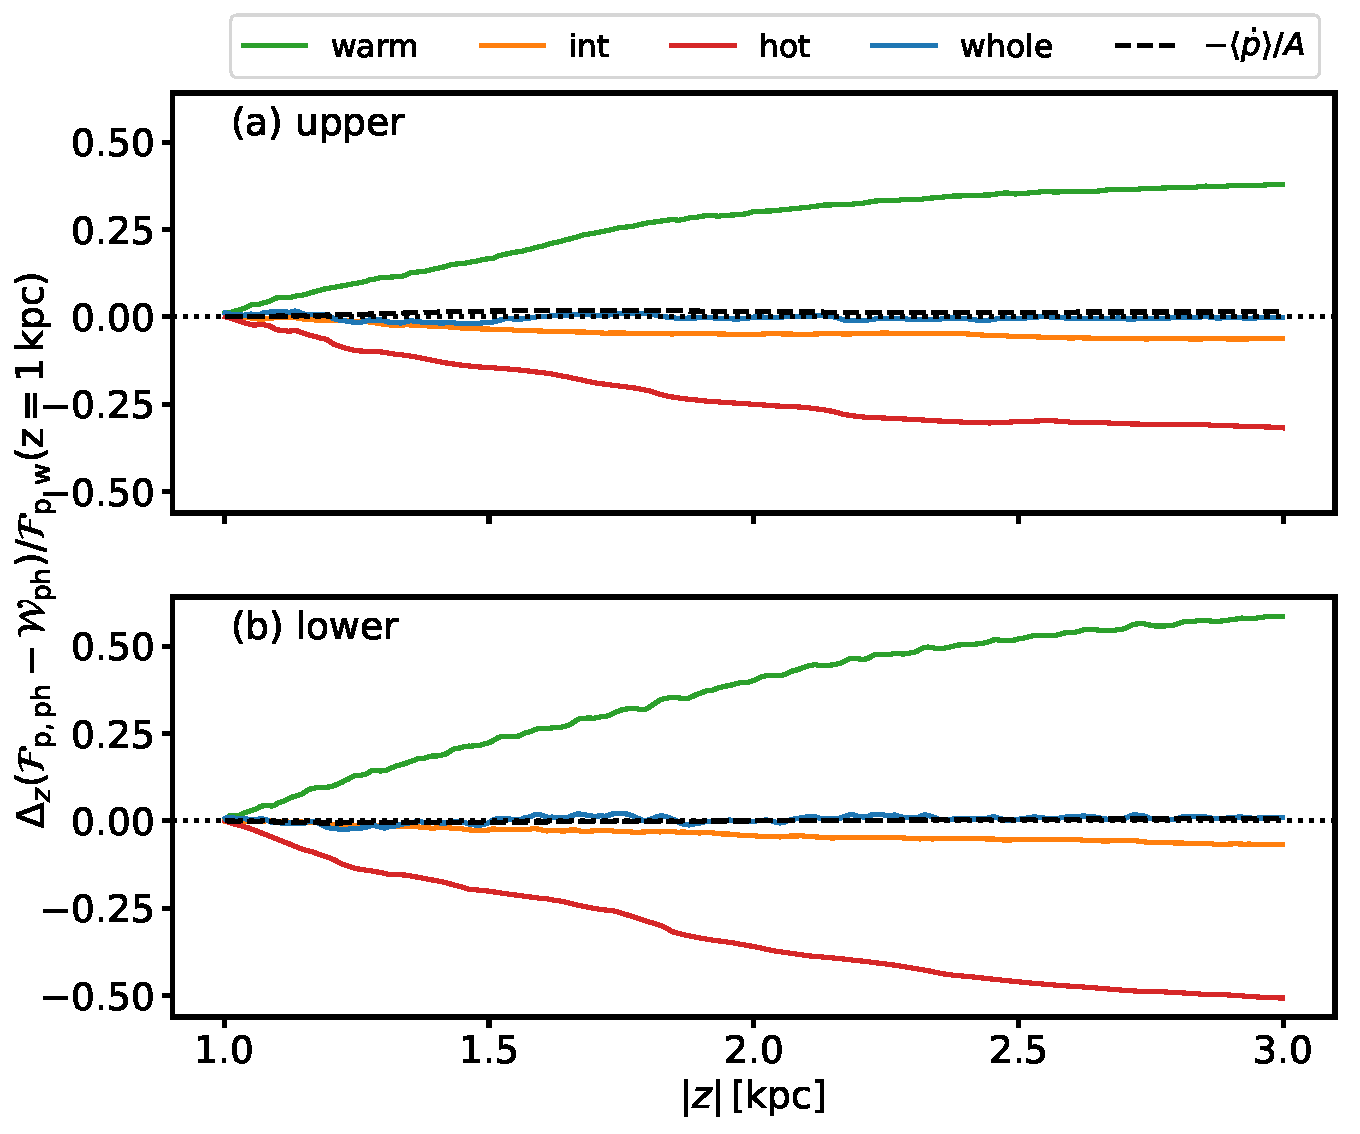
\includegraphics[width=0.9\textwidth]{momentum_conservation.pdf}
	\caption{Same as Figure~\ref{fig:mcons}, but for the net momentum flux difference by taking into account the flux loss by its own weight. Note that the net momentum change is nearly zero as the total not momentum flux difference.}
	\label{fig:pcons}
\end{figure*}
\begin{figure*}
	\centering
	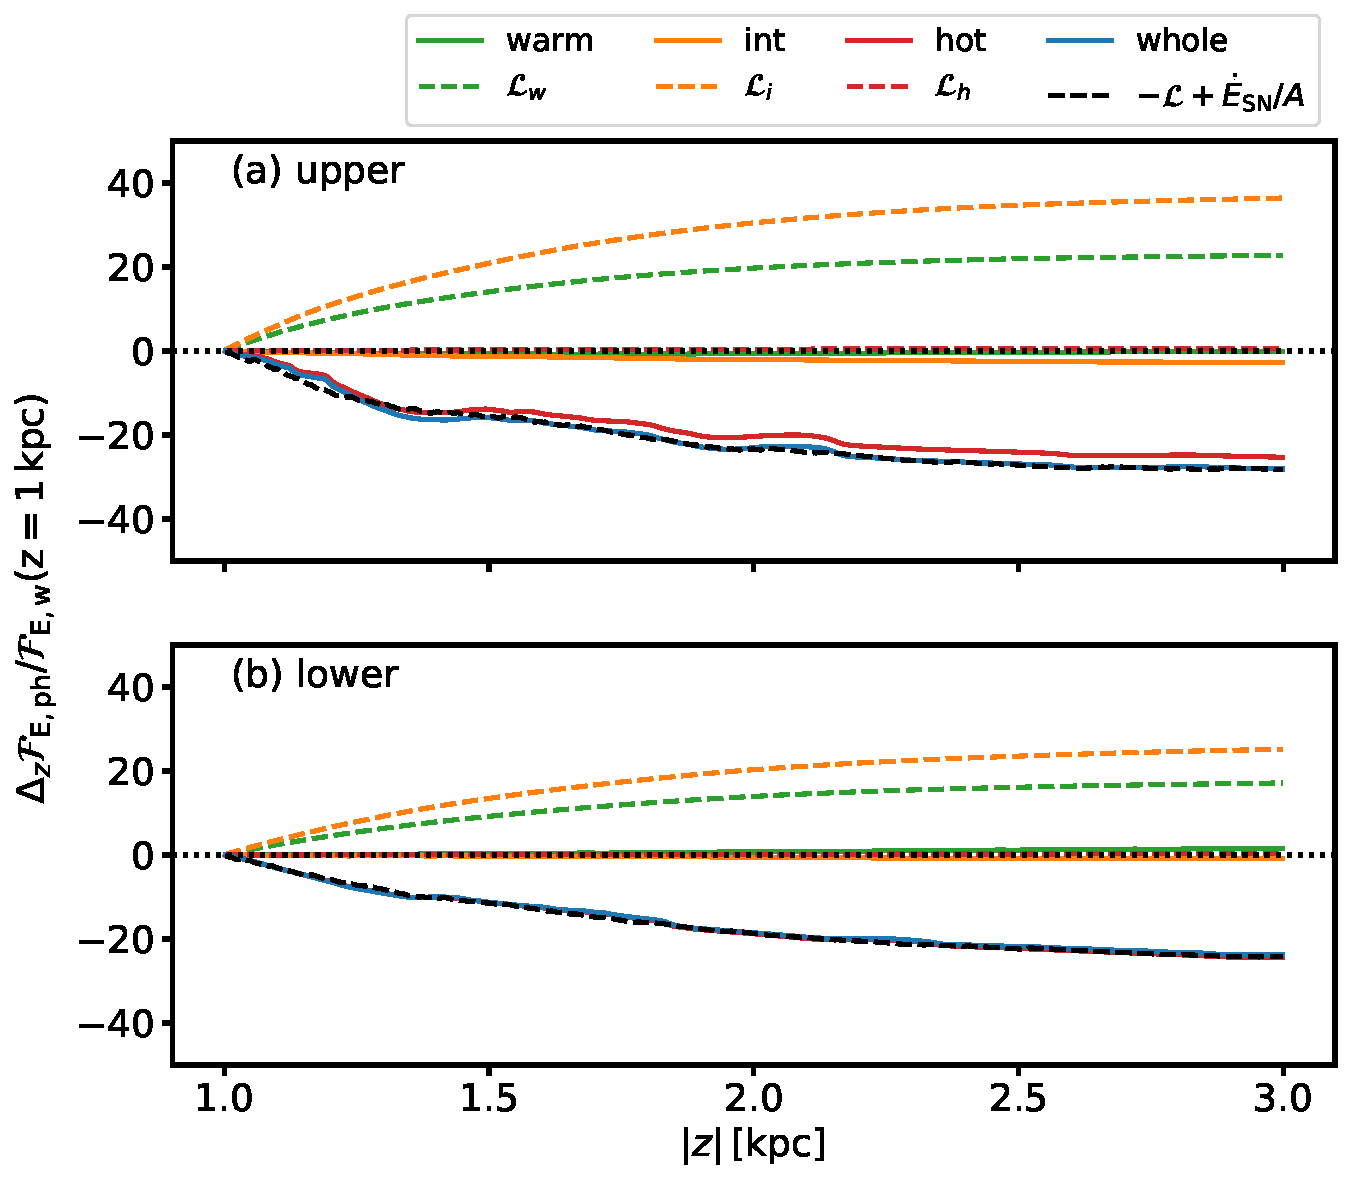
\includegraphics[width=0.9\textwidth]{energy_conservation.pdf}
	\caption{Same as Figure~\ref{fig:mcons}, but for the energy flux. In addition, the net cooling rate per unit area of each thermal gas phase is shown as dashed lines. The black dashed line denotes the total energy source term of the energy equation including the net cooling and direct SN energy injection, which matches the net energy flux change of the whole gas excellently. Note that the range of the y-axis is about two orders of magnitude larger than that in Figures~\ref{fig:mcons} and \ref{fig:pcons}.}
	\label{fig:econs}
\end{figure*}

In order to understand the evolution of multiphase outflows more completely, let us consider the conservation of mass, momentum, and energy with full hydrodynamics equations (we neglect magnetic fields here as we already see that the magnetic field contribution is negligible). We first take the horizontal average for each thermal phase and the temporal average for time range of $t\in(t_1,t_2)$ as defined in Equations (\ref{eqn:havg}) and (\ref{eqn:tavg}). Then, we further take vertical integration from $z=\pm z_i$, where $z_i$=1kpc, to a certain height $z$. The set of hydrodynamics equations now becomes
\begin{equation}
\sum_{\rm ph}\sbrackets{\abrackets{\dot{M}}_{\rm ph} + \Delta_z\mathcal{F}_{\rm M, ph}A}= 0,
\label{eqn:mcons}
\end{equation}
\begin{equation}\label{eqn:pcons}
\sum_{\rm ph} \sbrackets{\abrackets{\dot{p}}_{\rm ph} + 
 \rbrackets{ \Delta_z\mathcal{F}_{\rm p, ph} - \Delta_z\mathcal{W}_{\rm ph}}A} =0,
\end{equation}
\begin{equation}\label{eqn:econs}
\sum_{\rm ph} \sbrackets{\abrackets{\dot{E}}_{\rm ph} +
\Delta_z\mathcal{F}_{\rm E, ph}A}= -\mathcal{L}_{\rm ph}A+ \dot{E}_{\rm SN},
\end{equation}
where the rate of change in mass within the volume of interest is defined by
\begin{equation}\label{eqn:mdot}
    \abrackets{\dot{M}}_{\rm ph} \equiv \sum_{z'=z_i}^{z}
    \abrackets{\pderiv{\rho}{t}}_{\rm ph}\Delta z,
\end{equation}
while $\dot{p}$ and $\dot{E}$ are defined similarly by replacing $\rho$ with $\rho v_z$ and $\rho v^2/2+P_{\rm th}/(\gamma-1)$, respectively, where $\gamma=5/3$, is the adiabatic index.
The mass and energy fluxes are respectively defined by
$\mathcal{F}_{\rm M,ph}\equiv \abrackets{\rho v_z}_{\rm ph}$ 
and $\mathcal{F}_{\rm E,ph}\equiv \abrackets{\rho v_z\mathcal{B}}_{\rm ph}$,
where the Bernoulli parameter is defined by
\begin{equation}\label{eqn:Bernoulli}
\mathcal{B} \equiv \frac{v^2}{2} + \frac{\gamma}{\gamma -1} \frac{P_{\rm th}}{\rho} + \Phi.
\end{equation}
The momentum flux $\mathcal{F}_{\rm p, ph}$ and weight of gas $\mathcal{W}_{\rm ph}$ are defined by Equations (\ref{eqn:Fp}) and (\ref{eqn:weight}).
The source terms in Equation (\ref{eqn:econs}) are
energy loss by cooling $\mathcal{L}_{\rm ph}\equiv \sum_{z'=z_i}^{z}\abrackets{n^2\Lambda(T)-n\Gamma}_{\rm ph}(z')\Delta z$ and gain by 
direct SN energy injection $\dot{E}_{\rm SN} \equiv 10^{51}\erg N_{\rm SN}/t_{\rm bin}$. $\Delta_z$ denote the difference between the height of interest ($z$) and outflow launching ($z_i$), and $A=L_xL_y$ is the total area of the horizontal plane.

The first term in each equation (including summation over the phases) is the net change of total mass, momentum, and energy during the time interval we consider, which would be zero if the system is in a steady state. Due to the dynamic and bursty nature of the simulation, the steady state assumption within the volume we are analyzing is not always satisfied even after the long temporal averaging ($t_1=200\Myr$ and $t_2=550\Myr$). We thus keep this term to demonstrate how significant the unsteady behavior is. The total mass difference can be particularly large compared to the mass flux term. Although we consider the volume far from the midplane $|z|>1\kpc$, there is still direct SN energy injection due to SNe from runaways, which serves as a source term in the energy equation.

\subsection{Simulation Results\label{sec:flux_simulation}}
Figure~\ref{fig:mcons} plots the mass flux differences between the height of interest ($z$) and launching ($z_i$) for each thermal phase as well as the sum of all phases. We can see that there is net mass increase (positive flux difference for the whole gas) for this particular time interval. We emphasize that the amount of the net mass increase/decrease is time dependent. Although we cover long enough time interval to discuss a quasi-steady state behavior of outflows, it covers only a few dominant fountain cycles (see Figure~\ref{fig:mflux}) so that the net mass change can still be substantial unless the time interval encloses complete cycles. Our time interval is chosen to roughly begin with one breakout and end with the final inflow, but it cannot be perfect. The net changes in momentum and energy are negligible because the hotter and faster phase dominates momentum and energy.

Despite the time dependent net mass flux, Figure~\ref{fig:mcons} shows two robust features of the mass flux difference; (1) hot gas flux is nearly constant ($\Delta_z \mathcal{F}_{\rm M,h} = 0$) and (2) intermediate gas flux is decreased ($\Delta_z \mathcal{F}_{\rm M,i} < 0$). Note also that the net mass change is mostly due to the mass change in the warm phase ($\abrackets{\dot{M}}\approx\abrackets{\dot{M}}_{\rm w}$. Therefore, the amount that has been decreased from the intermediate phase must be added to the warm phase ($\abrackets{\dot{M}}_{\rm w} + \Delta_z \mathcal{F}_{\rm M,w}A = - \Delta_z \mathcal{F}_{\rm M,i}A$. Over the height range we consider here, the warm phase gains mass flux from the intermediate phase nearly continuously, and the total gain is 50\%-100\% of the mass flux of the warm phase at the launching. This reinforces the simplest idea applied to explain the discrepancy between ballistic model and simulation result in Section~\ref{subsec:bal_comparison}. The phase transition from the intermediate phase to the warm phase indeed occurs and substantial, but the excess of high velocity component in the warm phase is not a direct consequence of this phase transition as Figure~\ref{fig:ballistic_warm_int} demonstrates.

Next, we investigate momentum exchanges between phases. Figure~\ref{fig:pcons} plots the ``net'' momentum flux difference $\Delta_z(\mathcal{F}_{\rm p, ph} - \mathcal{W}_{\rm ph})$ rather than the momentum flux itself, which is always decreasing as the outflow climbs up the gravitational potential well $\Delta_z\mathcal{F}_{\rm p,ph} < 0$. The total net momentum flux difference is nearly zero since the vertical equilibrium holds at every heights as we see in Figure~\ref{fig:vertical_equilibrium}. However, the significant momentum flux loss occurs in the hot phase, which is clearly appeared as a gain in the warm phase. Although there is net loss in the intermediate phase as well (mainly due to direct phase transition as seen in Figure~\ref{fig:mcons}), the amount of the mass flux contribution from the intermediate phase to the warm phase is negligible compared to that from the hot phase. 
The total net gain of the warm phase momentum flux is about 50\% of its original momentum flux, which is comparable to the loss in the hot phase. The momentum flux of the warm phase is dominated by the turbulent term, while the turbulent and thermal terms of the hot phase are similar.

Lastly, Figure~\ref{fig:econs} plots the energy flux difference along with the total cooling and SN energy injection rate. The energy flux of the hot gas is huge compared to that in the warm phase and drained by the other phases ($\Delta_z \mathcal{F}_{\rm E,h}<0$). Also, the amount of energy injected by SN exploded within this volume is comparable to the hot gas energy flux loss. However, there is no significant increase of the energy flux in both warm and intermediate phases. Instead, cooling in both phases are comparable to the hot energy flux loss and SN energy injection ($\dot{E}_{\rm SN}-\Delta_z \mathcal{F}_{\rm E,h}A = (\mathcal{L}_{\rm w}+\mathcal{L}_{\rm w})A$.

In summary, from Figures~\ref{fig:mcons}-\ref{fig:econs}, we conclude that the warm phase gains mass flux from the intermediate phase and momentum flux from the hot phase. Although the energy flux available in the hot gas is enormous, this is not efficiently transferred to the other phase due to very efficient cooling in both warm and intermediate phases. The energy transfer between the hot and warm phases can occur by mixing or shocks. Both routes are mostly imparting thermal energy to the warm phase, which is quickly radiated away, without increasing kinetic energy of the warm phase much. The direct acceleration due to the hot phase momentum flux gradient is effective to increase the warm phase momentum flux. This makes overall interaction between phases minimal; only about a factor of 1.5-2 increase in the mass and momentum fluxes of the warm phase over $2\kpc$ compared to its steady-state injection fluxes.

\subsection{Size of Warm Cloud}\label{sec:flux_Rcl}
\begin{figure*}
	\centering
 	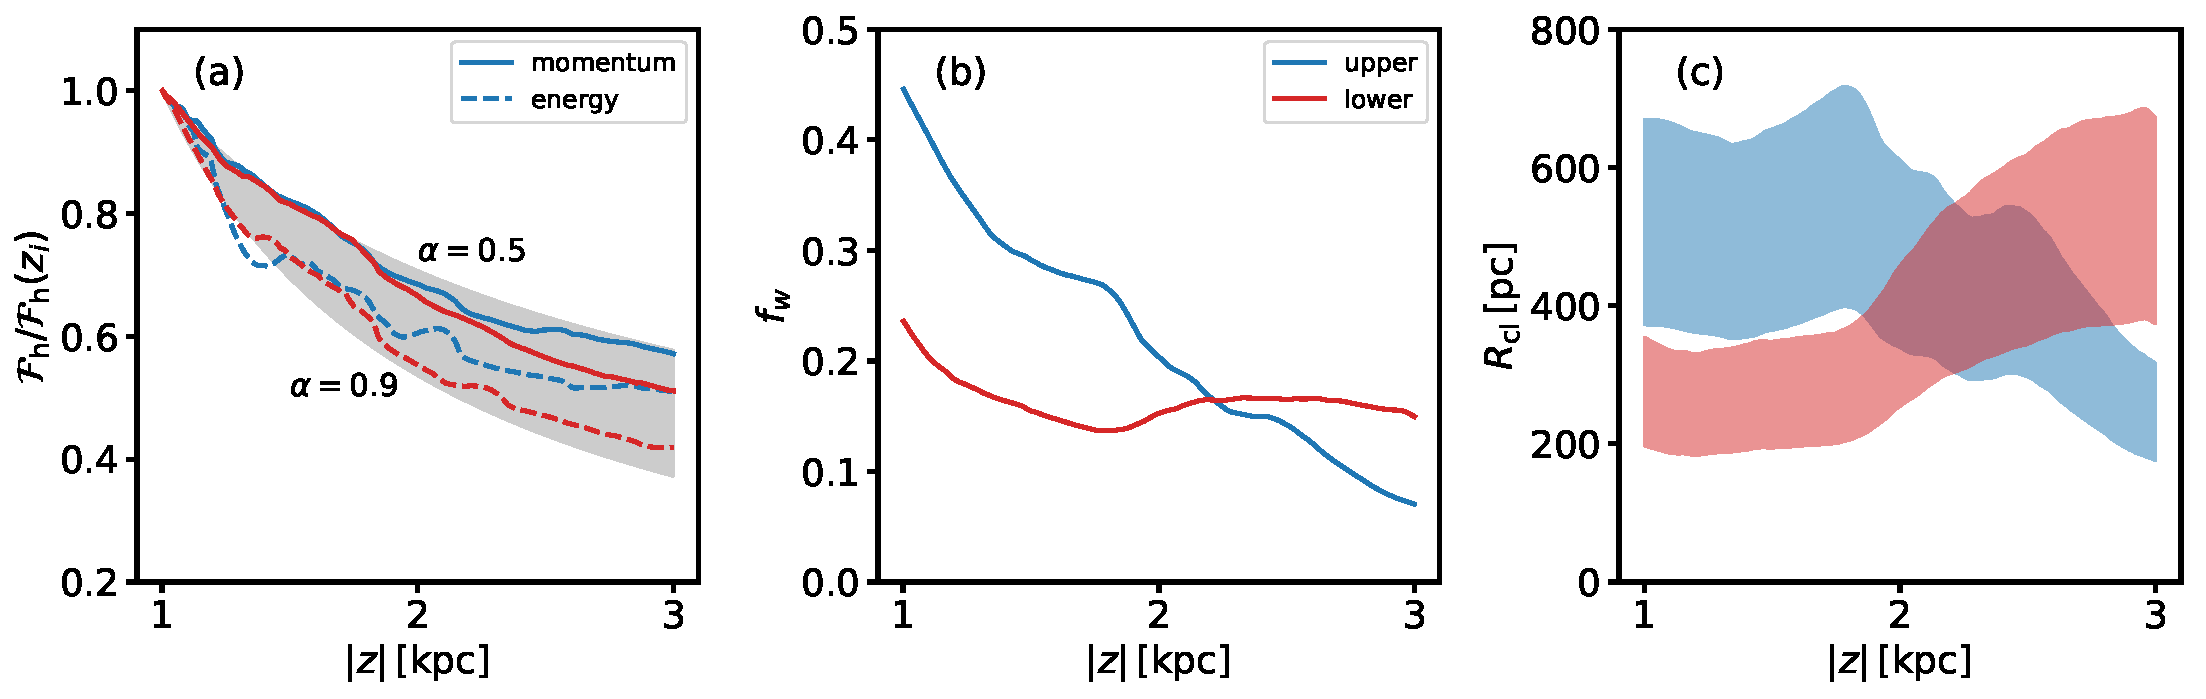
\includegraphics[width=\textwidth]{Rcl.pdf}
	\caption{{\bf (a)} Normalized flux profiles of momentum (solid) and energy (dashed) for the upper (blue) and lower (red) sides of the disk. Grey shaded region encloses a simplified model $(z/z_i)^{-\alpha}$ with a range of $\alpha=0.5$ to 0.9. 
	{\bf (b)} Volume filling factor profiles of the warm phase.
	{\bf (c)} Effective size of warm clouds $R_{\rm cl}$ derived by Equation (\ref{eqn:Rcl}. The shaded area covers the range of $\alpha$ we adopt in the panel (a). Larger $R_{\rm cl}$ corresponds to smaller $\alpha$. Note that the size of cloud is generally large so that the warm phase is likely to interact with the hot winds as a single entity rather than many small cloudlets.}
	\label{fig:rcl}
\end{figure*}

We now understand that the interaction between warm and hot phases occurs mainly due to the momentum exchange, which is also the main mechanism to keep the high velocity component in the warm phase. In this section, we calculate the effective size of warm clouds to quantify the overall type of the warm-hot interaction; are the hot winds interacting with many small cloudlets or a few big clouds? Based on simple assumptions that (1) the warm gas is in the form of spherical clouds with radius $R_{\rm cl}$ and (2) the hot gas flux is ``absorbed'' the warm clouds due to interaction, the flux loss of the hot gas can be written as
\begin{eqnarray}\label{eqn:dlnFh}
\deriv{\mathcal{F}_h}{z} = - n_{\rm cl} A_{\rm cl} \mathcal{F}_h,
\end{eqnarray}
where $\mathcal{F}_h$ can either be the momentum or energy flux. $A_{\rm cl}=\pi R_{\rm cl}^2$ is the cross-section of the warm cloud, and $n_{\rm cl}={M_{\rm w}}/{M_{\rm cl}V}$ is the number density of warm clouds,
where $M_{\rm w}=\rho_{\rm w} V_{\rm w}$ is the total mass of warm gas and $M_{cl}=4/3\pi R_{cl}^3\rho_{\rm w}$ is the mass of one cloud. 
We can rearrange Equation (\ref{eqn:dlnFh}) as
\begin{eqnarray}\label{eqn:Rcl}
\deriv{ \ln \mathcal{F}_h}{z} = - \frac{3}{4} \frac{f_w}{R_{\rm cl}},
\end{eqnarray}
where $f_w=V_w/V$ is the volume fraction of the warm phase. We note that the interaction (flux loss) is more efficient with a smaller cloud size as the effective cross-section increases with many small clouds.

In Figure~\ref{fig:rcl}(a), we first plot the normalized momentum (solid) and energy (dashed) fluxes, $\mathcal{F}_h/\mathcal{F}_h(z_i)$, from upper (blue) and lower (red) sides of the disk. Since the numerically measured flux is not a smooth function, the numerical derivative of it to obtain the LHS of Equation (\ref{eqn:Rcl}) gives very noisy results. For the sake of clarity of presentation, we simply adopt a functional form, $\mathcal{F}_h//\mathcal{F}_h(z_i)=(z/z_i)^{-\alpha}$ with a range of $\alpha$ from 0.5 to 0.9 that describes the general behavior of the flux loss (see the grey shaded region in Figure~\ref{fig:rcl}(a)). With the adopted model, $d\ln \mathcal{F}_h/dz=-\alpha/z$.

Using the volume fraction of the warm phase shown in Figure~\ref{fig:rcl}(b), we obtain the cloud size $R_{\rm cl}$ in Figure~\ref{fig:rcl}(c). Note that the larger $R_{\rm cl}$ corresponds to smaller $\alpha$ and less efficient interaction. The value of $R_{\rm cl}$ is generally large, $R_{\rm cl}\sim$ a few 100 pc, implying that the warm phase at the high-altitude regions that interacts with the hot winds exists more likely as one big entity rather than small cloudlets as seen in Figure~\ref{fig:slicenT}. This results in the minimal effective cross-section of the warm-hot interaction, which is consistent with the limited flux exchange between phases we see in Section~\ref{sec:flux_simulation}.



%%%%%%%%%%%%%%%%%%%%%%%%%%%%%%%%%%%%%%%%%%%%%%%%%%%%%%%%%%%%%%%%%%%%%%%%%%%%
\section{Summary \& Discussion}\label{sec:summary}

With a strong starburst, successful breakouts of superbubbles erupt energetic hot ($T>10^6\Kel$) and heavily loaded warm outflows ($T\sim10^4\Kel$) toward the circumgalactic space. Since star formation feedback drives outflows and quenches star formation by depositing momentum and energy within the disk ISM, the outflows are followed by inflows mostly in the form of the warm gas. While the hot winds simply flow away, the warm outflow/inflow (or usually called as fountains) partitions the significant amount of gas out of the disk scale height. Subsequent outflows meet the extraplanar gas blown out from the previous bursts (or from other parts of galactic disks) and interact with each other. Therefore, for complete understanding of galactic scale outflows, it is important to investigate how such multiphase outflows interact between phases and outflow cycles.

In this paper, we analyze magnetohydrodynamics simulations carried out by the TIGRESS numerical framework \citep{Kim&Ostriker17}, targeting the solar neighborhood condition. This simulation is ideal for the investigation of galactic outflows with complex interactions because: (1) it covers long time evolution and many star formation/feedback and outflow/inflow cycles; (2) star formation rates are self-regulated and SNe are placed in star clusters and runaways, giving self-consistent spatio-temporal correlations of feedback sources and surrounding ISM; and (3) the uniform spatial resolution employed in the simulation is necessary to correctly capture multiphase outflows and interaction between them numerically.
\citet{Kim&Ostriker18} presents the initial analysis of this model and quantifying the characteristics of the hot winds and warm fountains separately. In this paper, we extend this analysis including a simple ballistic model ignoring interaction and detailed consideration of flux exchanges between phases. Our main results are summarized as follows.

%CGK: I simply provide summary points; we can put discussions regarding each summary points.
\begin{enumerate}
    \item We demonstrate that the simulation shows bursty star formation and inflow/outflow cycles using the horizontally averaged space-time diagram of mass fluxes. We further take time range between 200 Myr and 550 Myr to construct time averaged profiles that are reasonably in a quasi-steady state, which are then used for the analysis.
    
    \item As the mass and momentum fluxes at the launching of outflows (we take $z_i=1\kpc\sim2H$) are dominated by the warm phase, the warm gas may evolve ballistically without significant interaction. In this case, the kinetic energy of the warm phase changes only due to the gravitational potential energy, which is dominated by the stellar disk and dark matter halo in the simulation. In Section~\ref{sec:ballistic}, we provide a formal framework to predict the velocity PDF at an arbitrary height $z$ from the initial velocity PDF at launching. The agreement between model and simulation outcome is quite good. Yet, there is general excess in the simulation outcome at high velocity component.
    
    \item To assess the degree of interaction between phases, we investigate the exchanges of the mass, momentum, and energy fluxes between thermal phases. We construct profiles of flux differences between the height of interest and launching. To isolate the exchange of fluxes between phases, it is important to factor out all other potential flux changes, including (1) the net mass change in the warm phase by the imperfectness of the steady-state assumption, (2) the momentum loss as the gas climbs up the gravitational potential, and (3) energy loss by cooling and gain by direct SN explosion. After taking these additional ``source'' terms, we can directly link between the loss of flux in one phase to the gain of flux in another phase.
    
    The mass flux of the hot phase is nearly constant. The loss in the intermediate phase is compensated by the gain in the warm phase. This is understood by the phase transition due to an efficient cooling in the intermediate phase. However, this cannot fully account the excess of the warm phase compared to the ballistic model.
    
    The ``net'' momentum flux difference shows loss in the hot phase and gain in the warm phase with negligible amount of loss in the intermediate phase. The amount of momentum transferred from the hot to warm phase is about 0.5 to 1 compared to the original momentum flux of the warm phase at the launching. 
    
    Interestingly, the energy flux of the hot phase shows huge loss, but no other phases gain it. With the direct energy injection from SNe exploded at high-altitude regions, about 50 times of the energy flux in the warm phase at the launching has lost from the hot phase. Very large amount of cooling in both warm and intermediate phases explains the loss without gain. 
    
    We conclude that the interaction between phases in the simulation generally means the loss of mass in the intermediate phase and energy in the hot phase and a little bit of momentum transfer from the hot to warm phase.
\end{enumerate}

%%%%%%%%%%%%%%%%%%%%%%%%%%%%%%%%%%%%%%%%%%%%%%%%%%%%%%%%%%%%%%%%%%%%%%%%%%%%
\begin{thebibliography}{999}

\bibitem[Armillotta et al.(2016)]{Armillotta+16} Armillotta, L., Fraternali, F., \& Marinacci, F.\ 2016, \mnras, 462, 4157 

\bibitem[Hu(2018)]{Hu19} Hu, Chia-Yu\ 2018, \mnras, 483, 3363 

\bibitem[Bolatto et al.(2013)]{Bolatto+13} Bolatto, A.~D., Warren, S.~R., Leroy, A.~K., et al.\ 2013, \nat, 499, 450 

%\bibitem[\protect\citeauthoryear{Bogdan et al}{2013}]{Bogdan2013} Bogdán, Á et al
%\ufhref[webgreen]{http://cdsads.u-strasbg.fr/abs/2013ApJ...772...97B}{ApJ, 772, 97B}

\bibitem[Bregman(1980)]{Bregman80} Bregman, J.~N.\ 1980, \apj, 236, 577 

\bibitem[Chen et al.(2010)]{Chen+10} Chen, Y.-M., Tremonti, C.~A., Heckman, T.~M., et al.\ 2010, \aj, 140, 445 

\bibitem[Chisholm et al.(2017)]{Chisholm+17} Chisholm, J., Tremonti, C.~A., Leitherer, C., \& Chen, Y.\ 2017, \mnras, 469, 4831 

\bibitem[Collins et al.(2002)]{Collins+02} Collins, J.~A., Benjamin, R.~A., \& Rand, R.~J.\ 2002, \apj, 578, 98 

\bibitem[Collins \& Rand(2001)]{Collins&Rand01} Collins, J.~A., \& Rand, R.~J.\ 2001, \apj, 551, 57 

\bibitem[Dekel \& Yuval(2006)]{Dekel&Yuval06} Dekel, Avishai; Birnboim, Yuval, \ 2006, \mnras, 368, 2 

%\bibitem[\protect\citeauthoryear{Dahlem et al}{1995}]{Dahlem1995}
%Dahlem, Michael; Lisenfeld, Ute; Golla, Gotz
%\ufhref[webgreen]{http://adsabs.harvard.edu/abs/1995ApJ...444..119D}{ApJ,}
%\ufhref[webgreen]{http://articles.adsabs.harvard.edu/full/1995ApJ...444..119D}{444, 119D}

%\bibitem[\protect\citeauthoryear{Dai et al}{2012}]{Dai2012}
%Dai, Xinyu; Anderson, Michael E.; Bregman, Joel N.; Miller, Jon M.
%\ufhref[webgreen]{http://adsabs.harvard.edu/abs/2012ApJ...755..107D}{ApJ, 755, 107D}

\bibitem[Ford et al.(2010)]{Ford+10} Ford, H.~A., Lockman, F.~J., \& McClure-Griffiths, N.~M.\ 2010, \apj, 722, 367 

\bibitem[Fraternali et al.(2002)]{Fraternali+02} Fraternali, F., van Moorsel, G., Sancisi, R., \& Oosterloo, T.\ 2002, \aj, 123, 3124 

\bibitem[Fraternali \& Binney(2006)]{Fraternali&Binney06} Fraternali, F., \& Binney, J.~J.\ 2006, \mnras, 366, 449 

\bibitem[Fraternali \& Binney(2008)]{Fraternali&Binney08} Fraternali, F., \& Binney, J.~J.\ 2008, \mnras, 386, 935 

\bibitem[Gatto et al.(2017)]{Gatto+17} Gatto, A., Walch, S., Naab, T., et al.\ 2017, \mnras, 466, 1903 

\bibitem[Gaensler et al.(2008)]{Gaensler+08} Gaensler, B.~M., Madsen, G.~J., Chatterjee, S., \& Mao, S.~A.\ 2008, \pasa, 25, 184 

\bibitem[Gronke \& Oh(2018)]{Gronke+18} Gronke, M., \& Oh, S.~P.\ 2018, \mnras, 480, L111 

\bibitem[Haffner et al.(2003)]{Haffner+03} Haffner, L.~M., Reynolds, R.~J., Tufte, S.~L., et al.\ 2003, \apjs, 149, 405 

\bibitem[Heald et al.(2006)]{Heald+06} Heald, G.~H., Rand, R.~J., Benjamin, R.~A., \& Bershady, M.~A.\ 2006, \apj, 647, 1018 

\bibitem[Heald et al.(2007)]{Heald+07} Heald, G.~H., Rand, R.~J., Benjamin, R.~A., \& Bershady, M.~A.\ 2007, \apj, 663, 933 

\bibitem[Heckman et al.(2015)]{Heckman+15} Heckman, T.~M., Alexandroff, R.~M., Borthakur, S., Overzier, R., \& Leitherer, C.\ 2015, \apj, 809, 147 

% \bibitem[Hoopes et al.(1999)]{Hoopes+99} Hoopes, C.~G., Walterbos, R.~A.~M., \& Rand, R.~J.\ 1999, \apj, 522, 669 

\bibitem[Iffrig \& Hennebelle(2017)]{Iffrig&Hennebelle17} Iffrig, O., \& Hennebelle, P.\ 2017, \aap, 604, A70 

\bibitem[Kalberla \& Kerp(2009)]{Kalberla&Kerp09} Kalberla, Peter M. W., Kerp, Jürgen 2017, ARA\&A, 47, 27 

%\ufhref[webgreen]{http://adsabs.harvard.edu/abs/2009ARA\%26A..47...27K}{ARA,}
%\ufhref[webgreen]{https://www.annualreviews.org/doi/full/10.1146/annurev-astro-082708-101823}{47, 27}

%\bibitem[Kim \& Ostriker(2015)]{Kim&Ostriker15a} Kim, C.-G., \& Ostriker, E.~C.\ 2015, \apj, 802, 99 

\bibitem[Kim et al.(2013)]{KOK13} Kim, C.-G., Ostriker, E.~C., \& Kim, W.-T.\ 2013, \apj, 776, 1 

\bibitem[Kim \& Ostriker(2015)]{KO15b} Kim, C.-G., \& Ostriker, E.~C.\ 2015, \apj, 815, 67 

\bibitem[Kim \& Ostriker(2017)]{Kim&Ostriker17} Kim, C.-G., \& Ostriker, E.~C.\ 2017, \apj, 846, 133 

\bibitem[Kim \& Ostriker(2018)]{Kim&Ostriker18} Kim, C.-G., \& Ostriker, E.~C.\ 2018, \apj, 853, 173 

\bibitem[Krishnarao et al.(2017)]{Krishnarao+17} Krishnarao, D., Haffner, L.~M., Benjamin, R.~A., Hill, A.~S., \& Barger, K.~A.\ 2017, \apj, 838, 43 

\bibitem[Kuijken \& Gilmore(1989)]{Kujiken&Gilmore} Kuijken, K., \& Gilmore, G.\ 1989, \mnras, 239, 605 

\bibitem[Leroy et al.(2015)]{Leroy+15} Leroy, A.~K., Bolatto, A.~D., Ostriker, E.~C., et al.\ 2015, \apj, 801, 25 

\bibitem[Lehner \& Christopher(2011)]{Lehner&Christoper11} Lehner, Nicolas; Howk, J. Christopher\ 2011, Science, 6058, 955

\bibitem[Lockman(2002)]{Lockman02} Lockman, F.~J.\ 2002, \apjl, 580, L47 

\bibitem[Marasco \& Fraternali(2011)]{Marasco&Fraternali11} Marasco, A., \& Fraternali, F.\ 2011, \aap, 525, A134 

\bibitem[Marasco et al.(2012)]{Marasco+12} Marasco, A., Fraternali, F., \& Binney, J.~J.\ 2012, \mnras, 419, 1107 

\bibitem[Marinacci et al.(2011)]{Marinacci2011}	
Marinacci, Federico; Fraternali, Filippo; Nipoti, Carlo; Binney, James; Ciotti, Luca; Londrillo, Pasquale\ 2011, \mnras, 415, 1534 

\bibitem[Hopkins et al.(2012)]{Hopkins12} Hopkins, P., F.,Quataert, E., \& Murray, N.,\ 2012, \mnras, 421, 3522

\bibitem[Matthews \& Wood(2003)]{Matthews&Wood03} Matthews, L.~D., \& Wood, K.\ 2003, \apj, 593, 721 

\bibitem[Oosterloo et al.(2007)]{Oosterloo+07} Oosterloo, T., Fraternali, F., \& Sancisi, R.\ 2007, \aj, 134, 1019 

\bibitem[Peek et al.(2011)]{Peek+11} Peek, J.~E.~G., Heiles, C., Douglas, K.~A., et al.\ 2011, \apjs, 194, 20 

\bibitem[Pillepich et al.(2018)]{Pillepich+18} Pillepich, A., Springel, V., Nelson, D., et al.\ 2018, \mnras, 473, 4077 

\bibitem[Reynolds(1991)]{Reynolds91} Reynolds, R.~J.\ 1991, The Interstellar Disk-Halo Connection in Galaxies, 144, 67

\bibitem[Rubin et al.(2012)]{Rubin+12} Rubin, Kate H. R.; Prochaska, J. Xavier; Koo, David C.; Phillips, Andrew C., 747, L26 

%\bibitem[\protect\citeauthoryear{Sancisi et al}{2008}]{Sancisi2008}
%Sancisi, Renzo; Fraternali, Filippo; Oosterloo, Tom; van der Hulst, Thijs
%\ufhref[webgreen]{http://adsabs.harvard.edu/abs/2008A\%26ARv..15..189S}{A \& ARv,}
%\ufhref[webgreen]{https://link.springer.com/article/10.1007\%2Fs00159-008-0010-0}{ 15, 189S}

\bibitem[Scannapieco \& Br{\"u}ggen(2015)]{Scannapieco&Bruggen15} Scannapieco, E., \& Br{\"u}ggen, M.\ 2015, \apj, 805, 158

\bibitem[Scannapieco et al.(2008)]{Scannapieco+09} 	
Scannapieco, Cecilia; Tissera, Patricia B.; White, Simon D. M.; Springel, Volker, 2008, \mnras, 389, 3 

\bibitem[Schaye et al.(2015)]{Schaye+15} Schaye, J., Crain, R.~A., Bower, R.~G., et al.\ 2015, \mnras, 446, 521 

\bibitem[Shapiro \& Field(1976)]{Shapiro&Field76} Shapiro, P.~R., \& Field, G.~B.\ 1976, \apj, 205, 762 

\bibitem[Sparre et al(2019)]{Sparre19} 	
Sparre, Martin; Pfrommer, Christoph; Vogelsberger, Mark, \mnras, 482, 5401

\bibitem[Strickland et al.(2004)]{Strickland+04} Strickland, D.~K., Heckman, T.~M., Colbert, E.~J.~M., Hoopes, C.~G., \& Weaver, K.~A.\ 2004, \apj, 606, 829 

\bibitem[Strickland \& Heckman(2007)]{Strickland&Heckman07} Strickland, D.~K., \& Heckman, T.~M.\ 2007, \apj, 658, 258 

\bibitem[Strickland \& Heckman(2009)]{Strickland&Heckman09} Strickland, D.~K., \& Heckman, T.~M.\ 2009, \apj, 697, 2030 

\bibitem[Teng et al.(2013)]{Teng+13} Teng, S.~H., Veilleux, S., \& Baker, A.~J.\ 2013, \apj, 765, 95 

\bibitem[Tumlinson et al.(2011)]{Tumlinson+11} Tumlinson, J., Thom, C., Werk, J.~K., et al.\ 2011, Science, 334, 948 

\bibitem[Tumlinson et al.(2017)]{Tumlinson+17} Tumlinson, J., Peeples, M., S,, Werk, J.~K., et al.\ 2017, ARA\&A

\bibitem[van Woerden et al.(2004)]{vanWoerden+04} van Woerden, H., Wakker, B.~P., Schwarz, U.~J., \& de Boer, K.~S.\ 2004, High Velocity Clouds, 312, 

\bibitem[Wakker \& van Woerden(1997)]{Wakker+97} Wakker, B. P.; van Woerden, H., \ 1997, AR\&A, 35, 217 

\bibitem[Wakker(2001)]{Wakker01} Wakker, B.~P.\ 2001, \apjs, 136, 463 

%\bibitem[\protect\citeauthoryear{Wakker and Savage}{2009}]{Wakker2009}
%Wakker, B. P.; Savage, B. D.
%\ufhref[webgreen]{http://adsabs.harvard.edu/abs/2009ApJS..182..378W}{ApJS, 182, 378}

\bibitem[Walter et al.(2002)]{Walter+02} Walter, F., Weiss, A., \& Scoville, N.\ 2002, \apjl, 580, L21 

\bibitem[Werk et al.(2014)]{Werk+14} Werk, J.~K., Prochaska, J.~X., Tumlinson, J., et al.\ 2014, \apj, 792, 8

\bibitem[Wong \& Blitz(2004)]{Wong&Blitz04} Wong, Tony; Blitz, Leo; Bosma, Albert\ 2005, \apj, 605, 183 

\bibitem[Zhag et al.(2013)]{Werk+14} 
Zhang, Dong; Thompson, Todd A.; Murray, Norman; Quataert, Eliot, \ 2013, \apj, 784, 93 

\bibitem[Zschaechner et al.(2011)]{Zschaechner+11} Zschaechner, L.~K., Rand, R.~J., Heald, G.~H., Gentile, G., \& Kamphuis, P.\ 2011, \apj, 740, 35 

\end{thebibliography}
\end{document}

% End of file `sample62.tex'.
